% vim: set spell spelllang=en tw=100 et sw=4 sts=4 foldmethod=marker foldmarker={{{,}}} :

\documentclass{beamer}

\usepackage{tikz}
\usepackage{xcolor}
\usepackage{complexity}
\usepackage{hyperref}
\usepackage{microtype}
\usepackage{amsmath}                   % \operatorname
\usepackage{amsfonts}                  % \mathcal
\usepackage{amssymb}                   % \nexists
\usepackage[vlined]{algorithm2e} % algorithms
\usepackage{centernot}
\usepackage{listings}
\usepackage{csquotes}
\usepackage{fancyvrb}
\usepackage{bussproofs}
\usepackage{multicol}
\usepackage{booktabs}

\RequirePackage[tt=false, type1=true]{libertine}
\RequirePackage[varqu]{zi4}
\RequirePackage[libertine]{newtxmath}
\RequirePackage[T1]{fontenc}

\lstdefinelanguage{opb}{morecomment=[l]*}
\lstdefinelanguage{veripb}{morecomment=[l]*, morekeywords=[2]{f, u, p, h, c},
keywordstyle=[2]\color{uofgcobalt}}
\lstdefinelanguage{C++H}[]{C++}{
    morekeywords=[2]{NoJustification, JustifyUsingRUP, JustifyExplicitly},
    keywordstyle=[2]\color{uofgcobalt}}
\lstdefinelanguage{MiniZinc}{
    morecomment=[l]\%,
    morekeywords={int, array, var, constraint, forall}}

\newcommand*{\rom}[1]{\emph{\romannumeral #1 \relax}}
\newcommand{\neighbourhood}{\operatorname{N}}
\newcommand{\vertexset}{\operatorname{V}}
\newcommand{\degree}{\operatorname{deg}}

\usetikzlibrary{shapes, arrows, shadows, calc, positioning, fit}
\usetikzlibrary{decorations.pathreplacing, decorations.pathmorphing, shapes.misc}
\usetikzlibrary{tikzmark, backgrounds}
\usetikzlibrary{trees}

\tikzset{processarrow/.style={->, very thick, decorate, decoration={snake, post length=0.5mm}}}
\tikzset{brace/.style={decorate, decoration={brace}, very thick}}

\definecolor{uofguniversityblue}{rgb}{0, 0.219608, 0.396078}

\definecolor{uofgheather}{rgb}{0.356863, 0.32549, 0.490196}
\definecolor{uofgaquamarine}{rgb}{0.603922, 0.72549, 0.678431}
\definecolor{uofgslate}{rgb}{0.309804, 0.34902, 0.380392}
\definecolor{uofgrose}{rgb}{0.823529, 0.470588, 0.709804}
\definecolor{uofgmocha}{rgb}{0.709804, 0.564706, 0.47451}
\definecolor{uofgsandstone}{rgb}{0.321569, 0.278431, 0.231373}
\definecolor{uofgforest}{rgb}{0, 0.2, 0.129412}
\definecolor{uofglawn}{rgb}{0.517647, 0.741176, 0}
\definecolor{uofgcobalt}{rgb}{0, 0.615686, 0.92549}
\definecolor{uofgturquoise}{rgb}{0, 0.709804, 0.819608}
\definecolor{uofgsunshine}{rgb}{1.0, 0.862745, 0.211765}
\definecolor{uofgpumpkin}{rgb}{1.0, 0.72549, 0.282353}
\definecolor{uofgthistle}{rgb}{0.584314, 0.070588, 0.447059}
\definecolor{uofgrust}{rgb}{0.603922, 0.227451, 0.023529}
\definecolor{uofgburgundy}{rgb}{0.490196, 0.133333, 0.223529}
\definecolor{uofgpillarbox}{rgb}{0.701961, 0.047059, 0}
\definecolor{uofglavendar}{rgb}{0.356863, 0.301961, 0.580392}

% {{{ theme things
\useoutertheme[footline=authortitle]{miniframes}
\useinnertheme{rectangles}

\setbeamerfont{block title}{size={}}
\setbeamerfont{title}{size=\large,series=\bfseries}
\setbeamerfont{section title}{size=\large,series=\mdseries}
\setbeamerfont{author}{size=\normalsize,series=\mdseries}
\setbeamercolor*{structure}{fg=uofguniversityblue}
\setbeamercolor*{palette primary}{use=structure,fg=black,bg=white}
\setbeamercolor*{palette secondary}{use=structure,fg=white,bg=uofgcobalt}
\setbeamercolor*{palette tertiary}{use=structure,fg=white,bg=uofguniversityblue}
\setbeamercolor*{palette quaternary}{fg=white,bg=black}

\setbeamercolor*{titlelike}{parent=palette primary}

\beamertemplatenavigationsymbolsempty

\setbeamertemplate{title page}
{
    \begin{tikzpicture}[remember picture, overlay]
        \node at (current page.north west) {
            \begin{tikzpicture}[remember picture, overlay]
                \fill [fill=uofguniversityblue, anchor=north west] (0, 0) rectangle (\paperwidth, -3.0cm);
            \end{tikzpicture}
        };

        \node (logo) [anchor=north east, shift={(-0.6cm,-0.2cm)}] at (current page.north east) {
            
\includegraphics[keepaspectratio=true,scale=0.5]{UoG_keyline.pdf}
        };

        \node (logo2) [anchor=north, below=0.2cm of logo.south] {
            
\includegraphics[keepaspectratio=true,scale=0.1]{RAEngWhite.pdf}
        };

        \coordinate (logos) at ($(logo.south)!0.5!(logo2.north)$);

        \node [anchor=west, xshift=0.2cm] at (current page.west |- logos) {
            \begin{minipage}{0.65\paperwidth}\raggedright
                {\usebeamerfont{title}\usebeamercolor[white]{}\inserttitle}\\[0.1cm]
                {\usebeamerfont{author}\usebeamercolor[white]{}\insertauthor}\\[0.1cm]
                {\usebeamerfont{author}\usebeamercolor[white]{}And numerous unindicted
                co-conspirators, including\\Bart Bogaerts, Stephan Gocht, Ross McBride,\\
                James Trimble, Jakob Nordstr\"{o}m, and Patrick Prosser}
            \end{minipage}
        };
    \end{tikzpicture}
}

\setbeamertemplate{section page}
{
    \begin{centering}
        \begin{beamercolorbox}[sep=12pt,center]{part title}
            \usebeamerfont{section title}\insertsection\par
        \end{beamercolorbox}
    \end{centering}
}

\newcommand{\frameofframes}{/}
\newcommand{\setframeofframes}[1]{\renewcommand{\frameofframes}{#1}}

\makeatletter
\setbeamertemplate{footline}
{%
    \begin{beamercolorbox}[colsep=1.5pt]{upper separation line foot}
    \end{beamercolorbox}
    \begin{beamercolorbox}[ht=2.5ex,dp=1.125ex,%
        leftskip=.3cm,rightskip=.3cm plus1fil]{author in head/foot}%
        \leavevmode{\usebeamerfont{author in head/foot}\insertshortauthor}%
        \hfill%
        {\usebeamerfont{institute in head/foot}\usebeamercolor[fg]{institute in head/foot}\insertshortinstitute}%
    \end{beamercolorbox}%
    \begin{beamercolorbox}[ht=2.5ex,dp=1.125ex,%
        leftskip=.3cm,rightskip=.3cm plus1fil]{title in head/foot}%
        {\usebeamerfont{title in head/foot}\insertshorttitle}%
        \hfill%
        {\usebeamerfont{frame number}\usebeamercolor[fg]{frame number}\insertframenumber~\frameofframes~\inserttotalframenumber}
    \end{beamercolorbox}%
    \begin{beamercolorbox}[colsep=1.5pt]{lower separation line foot}
    \end{beamercolorbox}
}

\makeatletter
\newenvironment{nearlyplainframe}[2][]{
    \def\beamer@entrycode{\vspace*{-\headheight}\vspace*{3pt}}
    \setbeamertemplate{headline}
    {%
        \begin{beamercolorbox}[colsep=1.5pt]{upper separation line head}
        \end{beamercolorbox}
        \begin{beamercolorbox}[ht=0.5ex,dp=0.125ex,%
            leftskip=.3cm,rightskip=.3cm plus1fil]{title in head/foot}%
        \end{beamercolorbox}%
        \begin{beamercolorbox}[ht=0.5ex,dp=0.125ex,%
            leftskip=.3cm,rightskip=.3cm plus1fil]{author in head/foot}%
        \end{beamercolorbox}%
        \begin{beamercolorbox}[colsep=1.5pt]{lower separation line head}
        \end{beamercolorbox}
        \vspace*{\headheight}
    }

    \setbeamertemplate{footline}
    {%
        \begin{beamercolorbox}[colsep=1.5pt]{upper separation line foot}
        \end{beamercolorbox}
        \begin{beamercolorbox}[ht=0.5ex,dp=0.125ex,%
            leftskip=.3cm,rightskip=.3cm plus1fil]{author in head/foot}%
        \end{beamercolorbox}%
        \begin{beamercolorbox}[ht=0.5ex,dp=0.125ex,%
            leftskip=.3cm,rightskip=.3cm plus1fil]{title in head/foot}%
        \end{beamercolorbox}%
        \begin{beamercolorbox}[colsep=1.5pt]{lower separation line foot}
        \end{beamercolorbox}
    }

    \begin{frame}[#1]{#2}
    }{
    \end{frame}
}
\makeatother

\makeatletter
\newenvironment{justborderframe}[2][]{
    \def\beamer@entrycode{\vspace*{-\headheight}}
    \setbeamertemplate{headline}
    {%
        \begin{beamercolorbox}[colsep=1.5pt]{upper separation line head}
        \end{beamercolorbox}
        \begin{beamercolorbox}[ht=0.5ex,dp=0.125ex,%
            leftskip=.3cm,rightskip=.3cm plus1fil]{title in head/foot}%
        \end{beamercolorbox}%
        \begin{beamercolorbox}[ht=0.5ex,dp=0.125ex,%
            leftskip=.3cm,rightskip=.3cm plus1fil]{author in head/foot}%
        \end{beamercolorbox}%
        \begin{beamercolorbox}[colsep=1.5pt]{lower separation line head}
        \end{beamercolorbox}
        \vspace*{\headheight}
    }

    \setbeamertemplate{footline}
    {%
        \begin{beamercolorbox}[colsep=1.5pt]{upper separation line foot}
        \end{beamercolorbox}
        \begin{beamercolorbox}[ht=0.5ex,dp=0.125ex,%
            leftskip=.3cm,rightskip=.3cm plus1fil]{author in head/foot}%
        \end{beamercolorbox}%
        \begin{beamercolorbox}[ht=0.5ex,dp=0.125ex,%
            leftskip=.3cm,rightskip=.3cm plus1fil]{title in head/foot}%
        \end{beamercolorbox}%
        \begin{beamercolorbox}[colsep=1.5pt]{lower separation line foot}
        \end{beamercolorbox}
    }

    \begin{frame}[#1]{}
    }{
    \end{frame}
}
\makeatother


% }}}

\author{Ciaran McCreesh}
\title{Proof Logging For Things That Aren't SAT}

\begin{document}

{
    \usebackgroundtemplate{
        \tikz[overlay, remember picture]
        \node[at=(current page.south), anchor=south, inner sep=0pt]{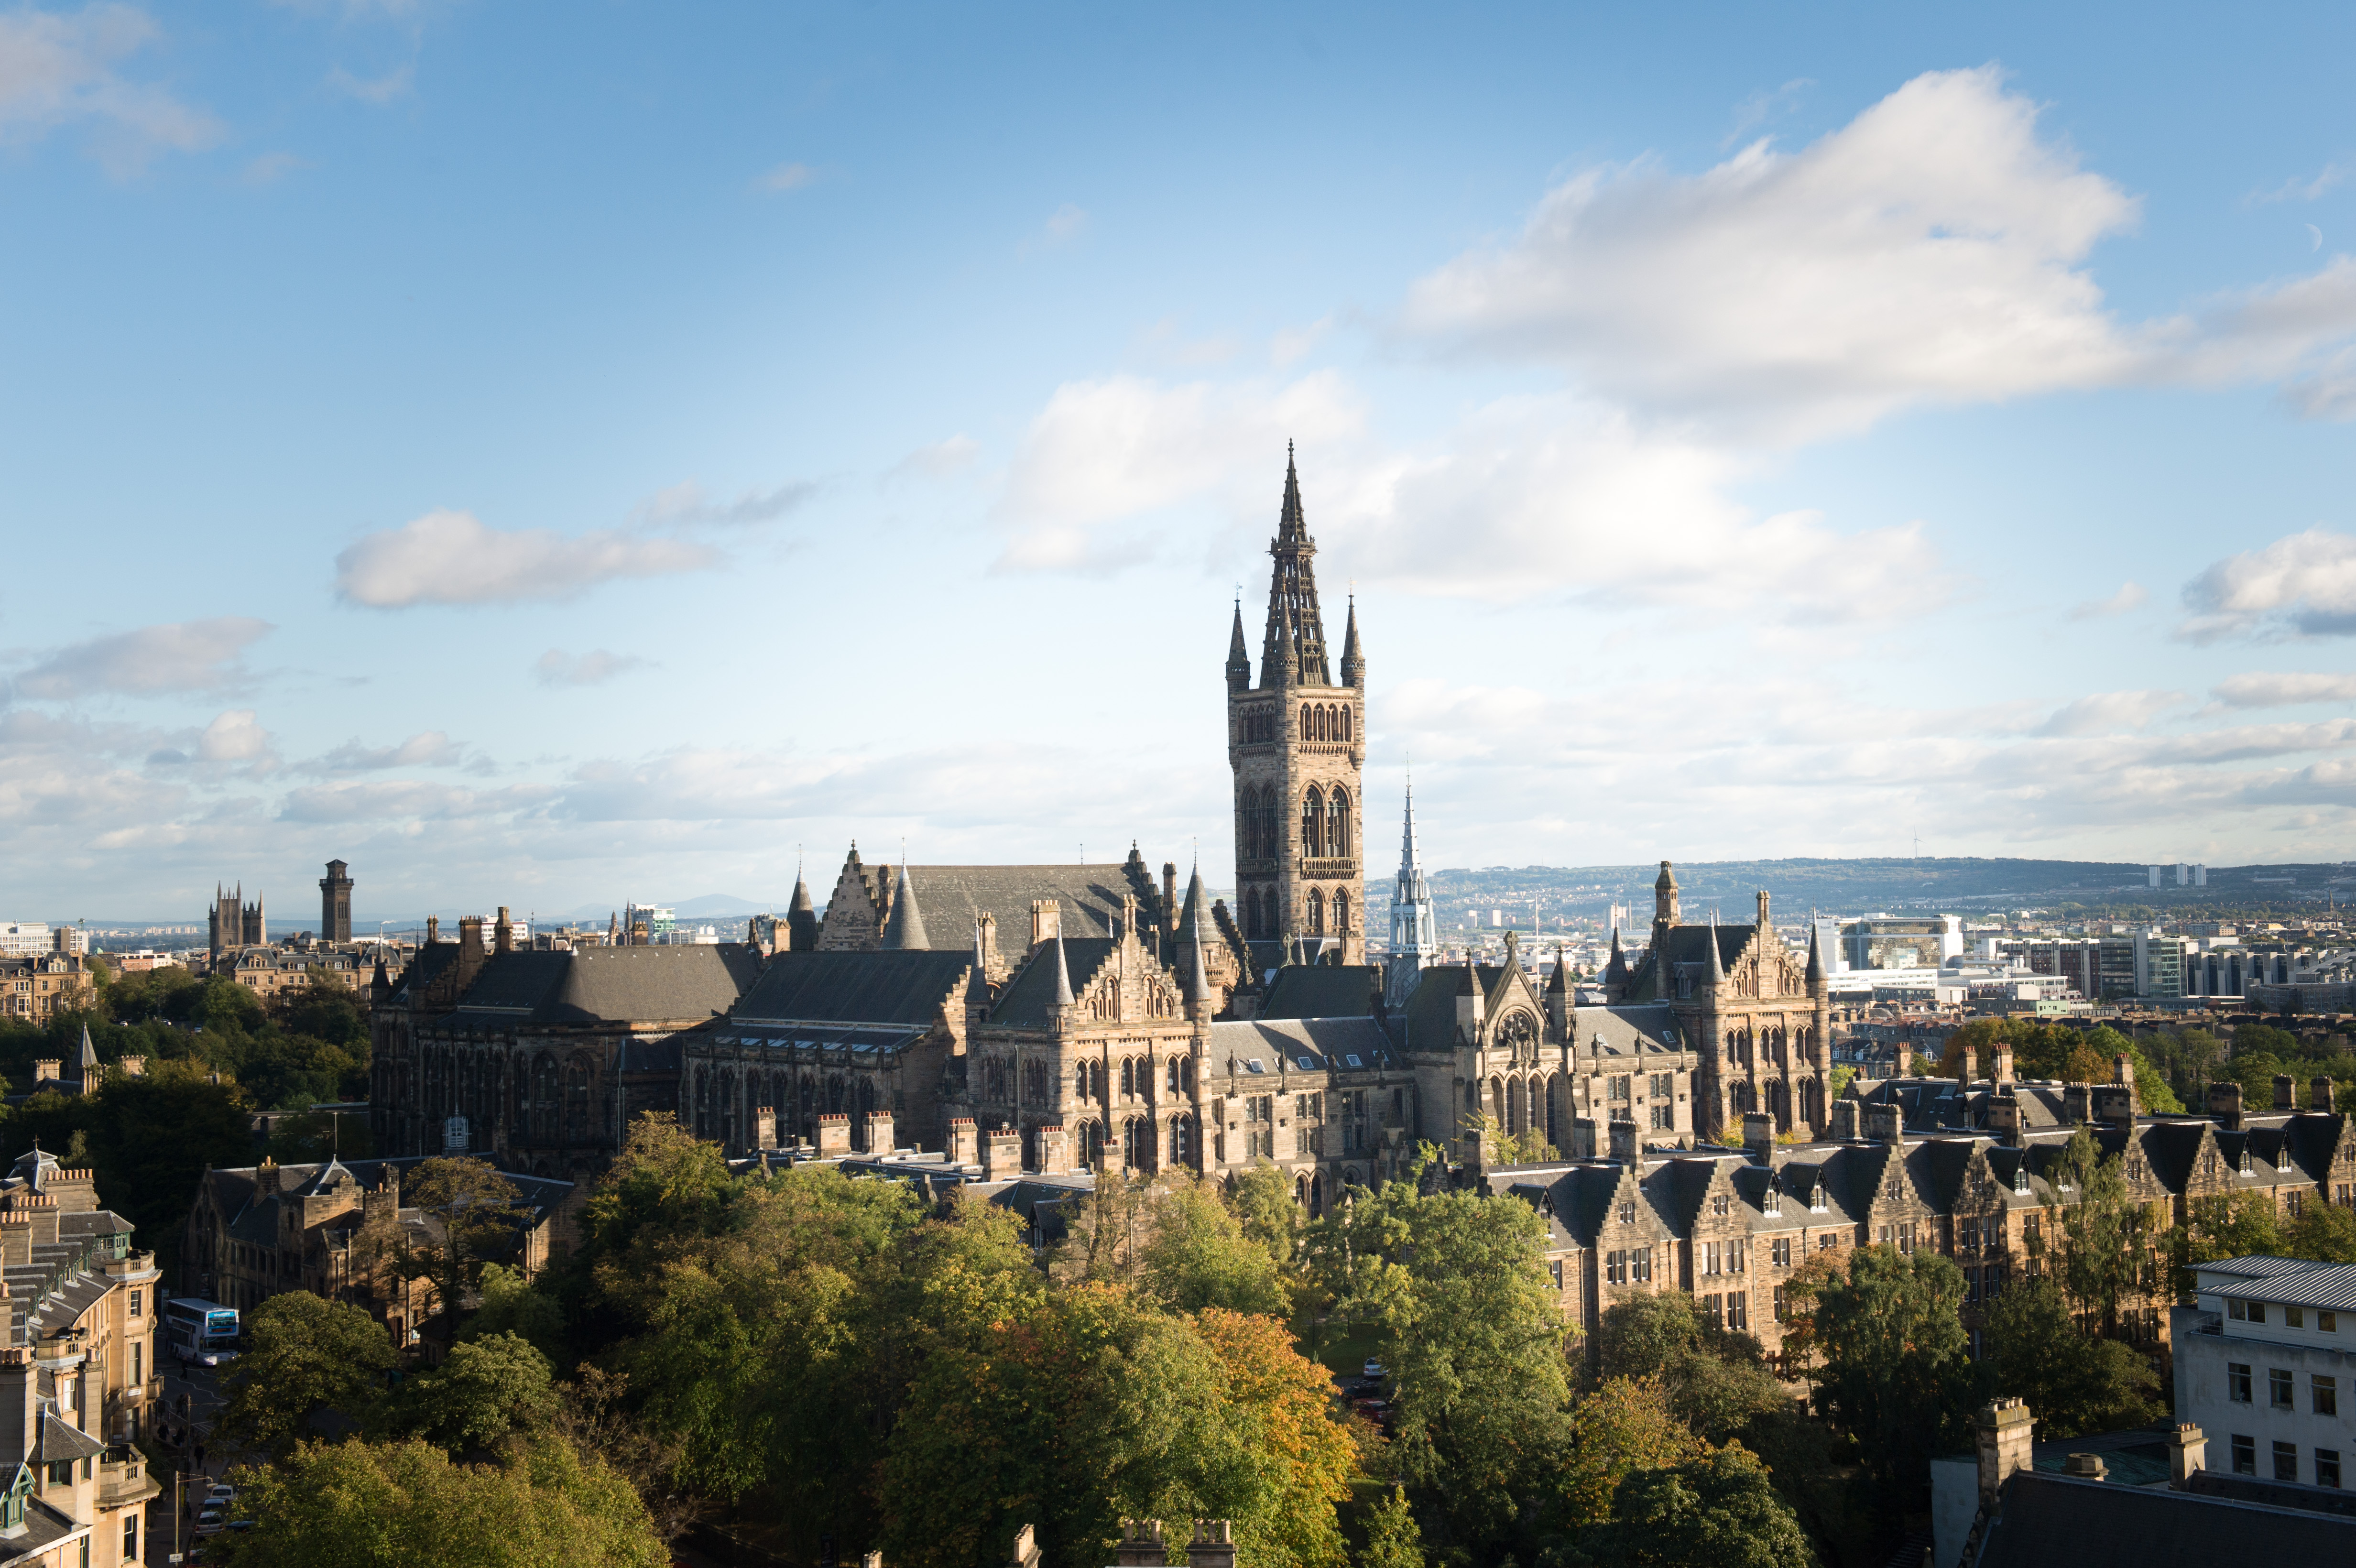
\includegraphics[keepaspectratio=true, height=\paperheight]{background.jpg}};
    }
    \begin{frame}[plain,noframenumbering]
        \titlepage
    \end{frame}
}

\section{Demotivation}

\begin{frame}{The Slide That Got Me Into Trouble}
    \begin{itemize}
        \item For somewhere between 0.1\% (my clique experiments) and 1.28\% (MiniZinc challenge
            2021) of instances, we get the wrong solution.
            \begin{itemize}
                \item False claims of unsatisfiability.
                \item False claims of optimality.
                \item Infeasible solutions produced.
                \item The same solver run on the same instance on the same hardware twice in a row
                    can claim both unsatisfiability and satisfiability.
            \end{itemize}
        \item This includes academic and commercial CP and MIP solvers.
        \item Extensive testing hasn't fixed this.
        \item Formal methods are far from being able to handle solvers.
        \item The situation for SAT solvers is somewhat better.
    \end{itemize}
\end{frame}

\section{Proof Logging}

\begin{frame}{Proof Logging}
    \begin{itemize}
        \item Certifying algorithms:
            \begin{itemize}
                \item Must produce a proof alongside an output.
                \item Verify outputs, not solvers.
                \item Unsat is the hard part.
            \end{itemize}
        \item A variety of formats for SAT: \ldots, DRAT, FRAT, \ldots.
        \item Huge success for SAT solving.
    \end{itemize}
\end{frame}

%%%\begin{frame}{Resolution Proofs}
%%%    \only<1>{
%%%    \begin{minipage}[c]{0.25\framewidth}
%%%        \textcolor{uofgcobalt}{\textbf{Model axioms}}
%%%    \end{minipage}\hfill\begin{minipage}[c]{0.70\framewidth}
%%%        \centering From the input
%%%    \end{minipage}\bigskip
%%%
%%%    \begin{minipage}[c]{0.25\framewidth}
%%%        \textcolor{uofgcobalt}{\textbf{Resolution}}
%%%    \end{minipage}\hfill\begin{minipage}[c]{0.70\framewidth}\begin{prooftree}
%%%        \AxiomC{$\textcolor{uofglawn}{x_1} \vee \textcolor{uofglawn}{x_2} \vee \ldots \vee
%%%        \textcolor{uofglawn}{x_i} \vee \textcolor{uofgpillarbox}{c}$}
%%%        \AxiomC{$\textcolor{uofgpillarbox}{\overline{c}} \vee \textcolor{uofgcobalt}{y_1} \vee
%%%        \textcolor{uofgcobalt}{y_2} \vee \ldots \textcolor{uofgcobalt}{y_j}$}
%%%        \BinaryInfC{$\textcolor{uofglawn}{x_1} \vee \textcolor{uofglawn}{x_2} \vee \ldots \vee
%%%        \textcolor{uofglawn}{x_i} \vee \textcolor{uofgcobalt}{y_1} \vee
%%%        \textcolor{uofgcobalt}{y_2} \vee \ldots \vee \textcolor{uofgcobalt}{y_j}$}
%%%    \end{prooftree}\end{minipage}
%%%
%%%    \bigskip
%%%
%%%    \begin{itemize}
%%%        \item To prove unsatisfiability: resolve until you reach the empty clause.
%%%    \end{itemize}
%%%}
%%%    \only<2->{
%%%        \begin{minipage}[c]{0.30\framewidth}
%%%            \begin{align}
%%%                & x \vee y \vee z \\
%%%                & \overline{x} \vee \overline{y} \vee \overline{z} \\
%%%                & \overline{x} \vee y \\
%%%                & \overline{x} \vee z \\
%%%                & x \vee \overline{y} \\
%%%                & x \vee \overline{z}
%%%            \end{align}
%%%        \end{minipage}\hfill\begin{minipage}[c]{0.60\framewidth}
%%%            \begin{align}
%%%                & 1, 5 \operatorname{on} y && x \vee z \\
%%%                & 6, 7 \operatorname{on} z && x \\
%%%                & 3, 8 \operatorname{on} x && y \\
%%%                & 4, 8 \operatorname{on} x && z \\
%%%                & 2, 8 \operatorname{on} x && \overline{y} \vee \overline{z} \\
%%%                & 9, 11 \operatorname{on} y && \overline{z} \\
%%%                & 10, 12 \operatorname{on} z && \emptyset
%%%            \end{align}
%%%
%%%        \end{minipage}
%%%    }
%%%\end{frame}
%%%
%%%\begin{frame}{Equisatisfiability and Completeness}
%%%    \begin{itemize}
%%%        \item Start with the constraints we're given.
%%%        \item At each step in a proof, add a new constraint which obviously doesn't affect satisfiability.
%%%        \item If we can derive contradiction, there were no solutions to the original problem.
%%%        \item Using resolution, we can always do this for any unsatisfiable SAT problem.
%%%    \end{itemize}
%%%\end{frame}
%%%
%%%\begin{frame}{Reverse Unit Propagation Proofs}
%%%    \begin{itemize}
%%%        \item Unit propagation:
%%%            \begin{itemize}
%%%                \item Look for a clause containing just one literal $\ell$.
%%%                \item Delete $\overline{\ell}$ from every other clause.
%%%                \item Repeat until you can't do anything.
%%%            \end{itemize}
%%%        \item Reverse unit propagation:
%%%            \begin{itemize}
%%%                \item Add the negation of a constraint $C$, and unit propagate.
%%%                \item If contradiction is reached, derive $C$.
%%%            \end{itemize}
%%%        \item Can rewrite to resolution in polynomial time.
%%%    \end{itemize}
%%%\end{frame}

\begin{frame}{World Domination Plans}
    \begin{itemize}
        \item Proof log all the things!
            \begin{itemize}
                \item OK, we'll stick to NP decision and optimisation for now.
            \end{itemize}
        \item Support both retrofitting and proof-driven development.
        \item Call it ``auditable solving''.
    \end{itemize}
\end{frame}

\begin{frame}{Opinionated Requirements}
    \begin{enumerate}
        \item Work with what solvers actually do, not idealised algorithms.
        \item No need for a new proof format for every new kind of algorithm.
            \begin{itemize}
                \item At least a hundred subgraph-finding algorithms, each of which does a different
                    kind of reasoning (colourings, neighbourhood degrees, paths, connectivity,
                    supplemental graphs, \ldots).
                    \begin{itemize}
                        \item The ``state of the art'' is often buggy\ldots
                    \end{itemize}
                \item Constraint programming has 423 different global constraints, many of which
                    have several different propagators.
                    \begin{itemize}
                        \item Some of which are buggy, and at least one has faulty theory behind it\ldots
                    \end{itemize}
            \end{itemize}
        \item Proof format must still be simple and well-founded.
            \begin{itemize}
                \item Need to be able to trust the verifier.
                \item Interactions between features can be subtle: even deletions aren't that easy
                    to get right.
            \end{itemize}
    \end{enumerate}
\end{frame}

\begin{frame}{Reusing DRAT Isn't Feasible}
    \begin{itemize}
        \item Closely tied to how MiniSAT works:
            \begin{itemize}
                \item Proofs are (mostly) sequences of learned clauses.
                \item Something special and strange happens to learned unit clauses.
            \end{itemize}
        \item Stronger reasoning is hard in theory and in practice.
        \item Preprocessing is possible (sometimes), but not easy.
            \begin{itemize}
                \item We need to do full-on reformulation, though.
            \end{itemize}
        \item Not clear how to do optimisation, enumeration, counting, \ldots
    \end{itemize}
\end{frame}

\begin{frame}[fragile]{Unexpected and Remarkable Claim}
    \only<1-3>{
    \begin{itemize}
        \item We can do everything we want with a proof format which is only slightly more
            sophisticated than DRAT.
        \item <2-> Using proof logs during development leads to faster development than not doing proof logging.
        \item <3-> You should make your students and postdocs adopt this technology right now.
    \end{itemize}}\begin{onlyenv}<4>
\tiny\begin{Verbatim}[commandchars=\\\{\},codes={\catcode`$=3\catcode`^=7}]
Dear Don,

A quick note on my experiences trying to solve the Sierpinski Gasket graphs:

I tried the latest version of Armin Biere's Kissat solver (
https://github.com/arminbiere/kissat ) using the most obvious SAT encoding, and
got the following run times:

S_6      0.02 seconds
S_7      0.12 seconds
S_8      0.73 seconds
S_9      3.92 seconds
S_10    27.81 seconds
S_11   160.37 seconds
S_12   716.13 seconds

[...]

Finally, I tried the program from the following paper. Unfortunately, it seems
to give incorrect answers for some of these instances.

\textcolor{red}{Citation removed to protect the guilty.}

Best regards,
James
\end{Verbatim}
    \end{onlyenv}
\end{frame}

%%%\begin{frame}{From CNF to Pseudo-Boolean Problems}
%%%    \begin{itemize}
%%%        \item A set of $\{ 0, 1 \}$-valued variables $x_i$, $1$ means true.
%%%        \item Constraints are linear inequalities \[
%%%                \sum_i c_i x_i \ge C
%%%            \]
%%%        \item Write $\overline{x}_i$ to mean $1 - x_i$.
%%%        \item Can rewrite CNF to pseudo-Boolean directly, \begin{align*}
%%%                & x_1 \vee \overline{x}_2 \vee x_3 & \leftrightarrow && x_1 + \overline{x}_2 + x_3 \ge 1
%%%        \end{align*}
%%%    \end{itemize}
%%%\end{frame}
%%%
%%%\begin{frame}{From Resolution to Cutting Planes}
%%%    \begin{minipage}[c]{0.35\framewidth}
%%%        \textcolor{uofgcobalt}{\textbf{Model axioms}}
%%%    \end{minipage}\hfill\begin{minipage}[c]{0.60\framewidth}
%%%        \centering From the input
%%%    \end{minipage}\bigskip
%%%
%%%    \begin{minipage}[c]{0.35\framewidth}
%%%        \textcolor{uofgcobalt}{\textbf{Literal axioms}}
%%%    \end{minipage}\hfill\begin{minipage}[c]{0.60\framewidth}\begin{prooftree}
%%%        \AxiomC{~}
%%%        \UnaryInfC{$\ell_i \ge 0$}
%%%    \end{prooftree}\end{minipage}\bigskip
%%%
%%%    \begin{minipage}[c]{0.35\framewidth}
%%%        \textcolor{uofgcobalt}{\textbf{Addition}}
%%%    \end{minipage}\hfill\begin{minipage}[c]{0.60\framewidth}\begin{prooftree}
%%%        \AxiomC{$\sum_i a_i \ell_i \ge A$}
%%%        \AxiomC{$\sum_i b_i \ell_i \ge B$}
%%%        \BinaryInfC{$\sum_i (a_i + b_i) \ell_i \ge A + B$}
%%%    \end{prooftree}\end{minipage}\bigskip
%%%
%%%    \begin{minipage}[c]{0.35\framewidth}
%%%        \textcolor{uofgcobalt}{\textbf{Multiplication}}\\
%%%        for any $c \in \mathbb{Z}$
%%%    \end{minipage}\hfill\begin{minipage}[c]{0.60\framewidth}\begin{prooftree}
%%%        \AxiomC{$\sum_i a_i \ell_i \ge A$}
%%%        \UnaryInfC{$\sum_i { c a_i \ell_i } \ge c A$}
%%%    \end{prooftree}\end{minipage}\bigskip
%%%
%%%    \begin{minipage}[c]{0.35\framewidth}
%%%        \textcolor{uofgcobalt}{\textbf{Division}}\\
%%%        for any $c \in \mathbb{N^+}$
%%%    \end{minipage}\hfill\begin{minipage}[c]{0.60\framewidth}\begin{prooftree}
%%%        \AxiomC{$\sum_i a_i \ell_i \ge A$}
%%%        \UnaryInfC{$\sum_i {\left\lceil \frac{a_i}{c} \right\rceil} \ell_i \ge \left\lceil \frac{A}{c} \right\rceil$}
%%%    \end{prooftree}\end{minipage}\bigskip
%%%\end{frame}
%%%
%%%\begin{frame}{Generalising Reverse Unit Propagation}
%%%\end{frame}

\section{Maximum Clique}

\begin{frame}{The Maximum Clique Problem}
    \begin{center}
    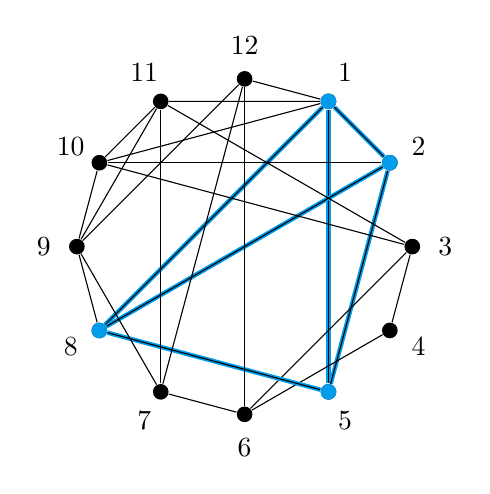
\begin{tikzpicture}
        \begin{scope}[scale=1.5]
        \newcount \myc
        \foreach \n in {3, 4, 6, 7, 9, 10, 11, 12}{
            \myc=\n \advance\myc by -1 \multiply\myc by -360 \divide\myc by 12 \advance\myc by 60.0
            \node[anchor=center] (L\n) at (\the\myc:1.7) {\n};
            \node[anchor=center, circle, fill=black, inner sep=2pt] (N\n) at (\the\myc:1.42) {};
        }
        \foreach \n in {1, 2, 5, 8}{
            \myc=\n \advance\myc by -1 \multiply\myc by -360 \divide\myc by 12 \advance\myc by 60.0
            \node[anchor=center] (L\n) at (\the\myc:1.7) {\n};
            \node<1>[anchor=center, circle, fill=black, inner sep=2pt] (N\n) at (\the\myc:1.42) {};
            \node<2>[anchor=center, circle, fill=uofgcobalt, inner sep=2pt] (N\n) at (\the\myc:1.42) {};
        }
        \draw <2> [ultra thick, color=uofgcobalt] (N1) -- (N2);
        \draw <2> [ultra thick, color=uofgcobalt] (N1) -- (N5);
        \draw <2> [ultra thick, color=uofgcobalt] (N1) -- (N8);
        \draw <1> (N1) -- (N2);
        \draw <1> (N1) -- (N5);
        \draw <1> (N1) -- (N8);
        \draw (N1) -- (N10);
        \draw (N1) -- (N11);
        \draw (N1) -- (N12);
        \draw <2> [ultra thick, color=uofgcobalt] (N2) -- (N5);
        \draw <2> [ultra thick, color=uofgcobalt] (N2) -- (N8);
        \draw <1> (N2) -- (N5);
        \draw <1> (N2) -- (N8);
        \draw (N2) -- (N10);
        \draw (N3) -- (N4);
        \draw (N3) -- (N6);
        \draw (N3) -- (N10);
        \draw (N3) -- (N11);
        \draw (N4) -- (N6);
        \draw <2> [ultra thick, color=uofgcobalt] (N5) -- (N8);
        \draw <1> (N5) -- (N8);
        \draw (N6) -- (N7);
        \draw (N6) -- (N12);
        \draw (N7) -- (N9);
        \draw (N7) -- (N11);
        \draw (N7) -- (N12);
        \draw (N8) -- (N9);
        \draw (N9) -- (N10);
        \draw (N9) -- (N11);
        \draw (N9) -- (N12);
        \draw (N10) -- (N11);
    \end{scope}
    \end{tikzpicture}
\end{center}
\end{frame}

\begin{frame}{The Certifying Process}
    \begin{itemize}
        \item Express the problem in pseudo-Boolean form (0/1 integer linear program; a superset of CNF):
            \begin{itemize}
                \item A set of $\{0, 1\}$-valued variables $x_i$.
                \item We define $\overline{x}_i = 1 - x_i$.
                \item Integer linear inequalities $\sum_{i} c_i x_i \ge C$.
                \item Optionally, an objective $\operatorname{min} \sum_{i} c_i x_i$.
            \end{itemize}
        \item Write this out as an OPB file.
        \item Provide a proof log for this OPB file.
            \begin{itemize}
                \item For unsat decision instances, prove $0 \ge 1$.
                \item Can also log sat decision instances, enumeration, and optimisation.
            \end{itemize}
        \item Feed the OPB file and the proof log to VeriPB.
    \end{itemize}
\end{frame}

\begin{frame}[t,fragile]{In Action\ldots}
\small\begin{Verbatim}[commandchars=\\\{\},codes={\catcode`$=3\catcode`^=7}]
\$ \textcolor{uofgcobalt}{./glasgow\textunderscore{}clique\textunderscore{}solver p\textunderscore{}hat500-2.clq}
nodes = 108217
clique = 37 59 63 68 71 102 124 133 137 150 160 186 206 222 231 238 269 300 302 308 342 348 349 368 381 383 384 404 412 425 432 445 457 480 489 500
runtime = 175ms
\end{Verbatim}

\begin{onlyenv}<2->\small\begin{Verbatim}[commandchars=\\\{\},codes={\catcode`$=3\catcode`^=7}]
\$ \textcolor{uofgcobalt}{./glasgow\textunderscore{}clique\textunderscore{}solver p\textunderscore{}hat500-2.clq --prove proof}
runtime = 16,347ms
\end{Verbatim}
\end{onlyenv}

\begin{onlyenv}<3->\small\begin{Verbatim}[commandchars=\\\{\},codes={\catcode`$=3\catcode`^=7}]
\$ \textcolor{uofgcobalt}{ls -lh proof.log proof.opb}
-rw-rw-r-- 1 ciaranm ciaranm 558M Aug 23 21:43 proof.log
-rw-rw-r-- 1 ciaranm ciaranm 1.4M Aug 23 21:42 proof.opb
\end{Verbatim}
\end{onlyenv}

\begin{onlyenv}<4->\small\begin{Verbatim}[commandchars=\\\{\},codes={\catcode`$=3\catcode`^=7}]
\$ \textcolor{uofgcobalt}{veripb proof.opb proof.log}
INFO:root:total time: 428.89s
maximal used database memory: 0.003 GB
Verification succeeded.
\end{Verbatim}
\end{onlyenv}
\end{frame}

\begin{frame}[fragile]{A Pseudo-Boolean Encoding}
    \begin{center}
    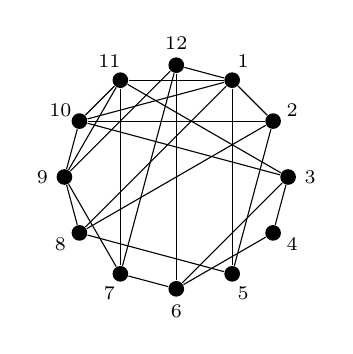
\begin{tikzpicture}
        \begin{scope}[every node/.style = {font=\scriptsize}]
        \newcount \myc
        \foreach \n in {3, 4, 6, 7, 9, 10, 11, 12}{
            \myc=\n \advance\myc by -1 \multiply\myc by -360 \divide\myc by 12 \advance\myc by 60.0
            \node[anchor=center] (L\n) at (\the\myc:1.7) {\n};
            \node[anchor=center, circle, fill=black, inner sep=2pt] (N\n) at (\the\myc:1.42) {};
        }
        \foreach \n in {1, 2, 5, 8}{
            \myc=\n \advance\myc by -1 \multiply\myc by -360 \divide\myc by 12 \advance\myc by 60.0
            \node[anchor=center] (L\n) at (\the\myc:1.7) {\n};
            \node[anchor=center, circle, fill=black, inner sep=2pt] (N\n) at (\the\myc:1.42) {};
        }
            \draw  (N1) -- (N2);
            \draw  (N1) -- (N5);
            \draw  (N1) -- (N8);
        \draw (N1) -- (N10);
        \draw (N1) -- (N11);
        \draw (N1) -- (N12);
            \draw  (N2) -- (N5);
            \draw  (N2) -- (N8);
        \draw (N2) -- (N10);
        \draw (N3) -- (N4);
        \draw (N3) -- (N6);
        \draw (N3) -- (N10);
        \draw (N3) -- (N11);
        \draw (N4) -- (N6);
            \draw  (N5) -- (N8);
        \draw (N6) -- (N7);
        \draw (N6) -- (N12);
        \draw (N7) -- (N9);
        \draw (N7) -- (N11);
        \draw (N7) -- (N12);
        \draw (N8) -- (N9);
        \draw (N9) -- (N10);
        \draw (N9) -- (N11);
        \draw (N9) -- (N12);
        \draw (N10) -- (N11);
    \end{scope}
    \end{tikzpicture}
\end{center}

\small\begin{Verbatim}[commandchars=\\\{\},codes={\catcode`$=3\catcode`^=7}]
\textcolor{uofgcobalt}{* #variable= 12 #constraint= 41}
min: -1 x1 -1 x2 -1 x3 -1 x4 \emph{\ldots{}and so on\ldots{}} -1 x11 -1 x12 ;
1 ~x3 1 ~x1 >= 1 ;
1 ~x3 1 ~x2 >= 1 ;
1 ~x4 1 ~x1 >= 1 ;
\textcolor{uofgcobalt}{* \ldots{}and a further 38 similar lines for the remaining non-edges}
\end{Verbatim}
\end{frame}

\begin{frame}{A Search Tree}
    \begin{center}
    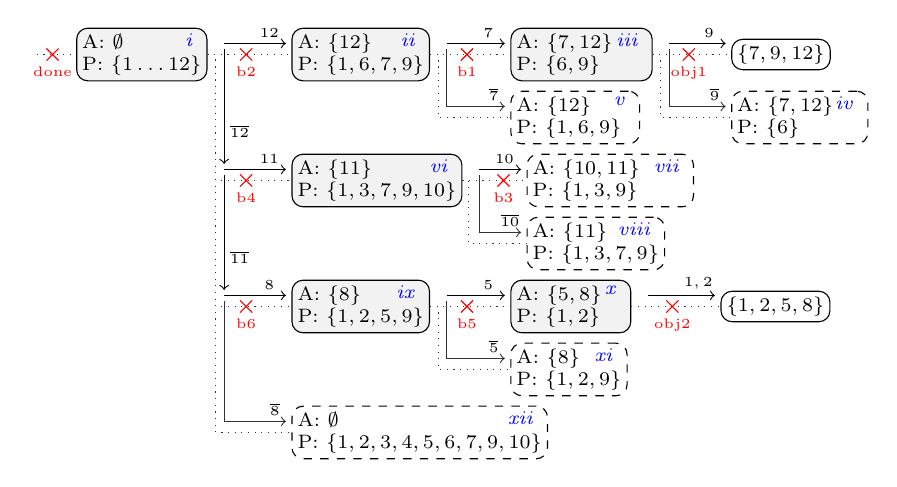
\begin{tikzpicture}
    \begin{scope}[
           color=black!80,
           dotted,
           grow via three points={one child at (1.9, 0) and two children at (1.9, 0) and (1.9, -0.8)},
           edge from parent path={(\tikzparentnode.east) -| ($(\tikzparentnode.east)!0.1!(\tikzchildnode.west)$) |- (\tikzchildnode.west)},
           every node/.style = {align=left, anchor=west, font=\scriptsize, inner sep=2pt, color=black, solid},
           branch/.style = {shape=rectangle, rounded corners, fill=gray!10, draw},
           notbranch/.style = {shape=rectangle, rounded corners, draw, dashed},
           sol/.style = {shape=rectangle, rounded corners, draw},
           state/.style = {color=blue},
           bt/.style = {color=red, font=\tiny, anchor=center},
           acceptarr/.style = {->, color=black, solid, transform canvas={yshift=0.4em}, shorten >=0.2em, shorten <=0.6em},
           rejectarr/.style = {->, solid, color=black, transform canvas={xshift=0.6em, yshift=0.4em}, shorten >=0.2em, shorten <=0.2em},
           rejectarrl/.style = {->, solid, transform canvas={xshift=0.6em, yshift=0.4em}, shorten >=0.8em, shorten <=0.2em},
           accept/.style = {font=\tiny, anchor=east, color=black, solid, pos=1.0, above=0cm, xshift=-0.8em},
           reject/.style = {anchor=north west, right=0cm, font=\tiny, black, pos=0.7},
           rejectl/.style = {anchor=east, above=0cm, font=\tiny, black, pos=1.0, xshift=-1.2em}
        ]
        \node (I) [branch] {A: $\emptyset$ \\ P: $\{1\ldots12\}$}
        child [] {
            node (A12) [branch] {A: $\{12\}$ \\ P: $\{1, 6, 7, 9\}$}
            child [] {
                node (A7A12) [branch] {A: $\{ 7, 12 \}$ \\ P: $\{ 6, 9 \}\phantom{, 1xx}$}
                child [] {
                    node (Sol1) [sol] {$\{7, 9, 12 \}$}
                    edge from parent node [bt, draw, cross out, pos=0.7] (sol1x) { }
                }
                child [] {
                    node (A7A12R9) [notbranch] {A: $\{ 7, 12 \}$ \\ P: $\{ 6 \}\phantom{xxxxx}$}
                }
                edge from parent node [bt, draw, cross out, pos=0.7] (bt1x) { }
            }
            child [] {
                node (A12R7) [notbranch] {A: $\{ 12 \}$ \\ P: $\{ 1, 6, 9 \}\phantom{x}$}
            }
            edge from parent node [bt, draw, cross out, pos=0.7] (bt2x) { }
        }
        child [missing] {}
        child [] {
            node (R12A11) [branch] {A: $\{11\}$ \\ P: $\{ 1, 3, 7, 9, 10 \}$}
            child [] {
                node (A10A11) [notbranch] {A: $\{10, 11\}$ \\ P: $\{ 1, 3, 9 \}\phantom{xxxx}$}
                edge from parent node [bt, draw, cross out, pos=0.8] (bt3x) { }
            }
            child [] {
                node (A11R10) [notbranch] {A: $\{11\}$ \\ P: $\{ 1, 3, 7, 9 \}$}
            }
            edge from parent node [bt, draw, cross out, pos=0.7] (bt4x) { }
        }
        child [missing] {}
        child [] {
            node (A8) [branch] {A: $\{8\}$ \\ P: $\{ 1, 2, 5, 9 \}$}
            child [] {
                node (A5A8) [branch] {A: $\{ 5, 8 \}$ \\ P: $\{ 1, 2 \}\phantom{xx}$}
                child [] {
                    node (Sol2) [sol] {$\{ 1, 2, 5, 8 \}$}
                    edge from parent node [bt, draw, cross out, pos=0.7] (sol2x) { }
                }
                edge from parent node [bt, draw, cross out, pos=0.7] (bt5x) { }
            }
            child [] {
                node (A8R5) [notbranch] {A: $\{ 8 \}$ \\ P: $\{ 1, 2, 9 \}$}
            }
            edge from parent node [bt, draw, cross out, pos=0.7] (bt6x) { }
        }
        child [missing] {}
        child [] {
            node (R8R11R12) [notbranch] {A: $\emptyset$ \\ P: $\{ 1, 2, 3, 4, 5, 6, 7, 9, 10 \}$}
        }
        ;

        \coordinate [left=0.5cm of I.west] (InLine);
        \draw (InLine) -- node [bt, draw, cross out, pos=0.4] (bt7x) { } (I.west);

        \node [bt, anchor=north, below=0cm of bt1x] {b1};
        \node [bt, anchor=north, below=0cm of bt2x] {b2};
        \node [bt, anchor=north, below=0cm of bt3x] {b3};
        \node [bt, anchor=north, below=0cm of bt4x] {b4};
        \node [bt, anchor=north, below=0cm of bt5x] {b5};
        \node [bt, anchor=north, below=0cm of bt6x] {b6};
        \node [bt, anchor=north, below=0cm of bt7x] {done};
        \node [bt, anchor=north, below=0cm of sol1x] {obj1};
        \node [bt, anchor=north, below=0cm of sol2x] {obj2};

        \draw [acceptarr] (I) -> node [accept] {$12$} (A12);
        \draw [acceptarr] (A12) -> node [accept] {$7$} (A7A12);
        \draw [acceptarr] (A7A12) -> node [accept] {$9$} (Sol1);
        \draw [acceptarr] (I.east |- R12A11.west) -> node [accept] {$11$} (R12A11);
        \draw [acceptarr] (I.east |- A8.west) -> node [accept] {$8$} (A8);
        \draw [acceptarr] (R12A11) -> node [accept] {$10$} (A10A11);
        \draw [acceptarr] (A8) -> node [accept] {$5$} (A5A8);
        \draw [acceptarr] (A5A8) -> node [accept] {$1, 2$} (Sol2);

        \draw [rejectarr] (I.east) -> node [reject] {$\overline{12}$} (I.east |- R12A11.east);
        \draw [rejectarr] (I.east |- R12A11.east) -> node [reject] {$\overline{11}$} (I.east |- A8.west);
        \draw [rejectarrl] (I.east |- A8.east) -- (I.east |- R8R11R12.west) -> node [rejectl] {$\overline{8}$} (R8R11R12.west);
        \draw [rejectarrl] (A12.east) -- (A12.east |- A12R7.east) -> node [rejectl] {$\overline{7}$} (A12R7.west);
        \draw [rejectarrl] (A7A12.east) -- (A7A12.east |- A7A12R9.east) -> node [rejectl] {$\overline{9}$} (A7A12R9.west);
        \draw [rejectarrl] (R12A11.east) -- (R12A11.east |- A11R10.east) -> node [rejectl] {$\overline{10}$} (A11R10.west);
        \draw [rejectarrl] (A8.east) -- (A8.east |- A8R5.east) -> node [rejectl] {$\overline{5}$} (A8R5.west);

        \node [state, anchor=north east] at (I.north east) { \rom{1} };
        \node [state, anchor=north east] at (A12.north east) { \rom{2} };
        \node [state, anchor=north east] at (A7A12.north east) { \rom{3} };
        \node [state, anchor=north east] at (A7A12R9.north east) { \rom{4} };
        \node [state, anchor=north east] at (A12R7.north east) { \rom{5} };
        \node [state, anchor=north east] at (R12A11.north east) { \rom{6} };
        \node [state, anchor=north east] at (A10A11.north east) { \rom{7} };
        \node [state, anchor=north east] at (A11R10.north east) { \rom{8} };
        \node [state, anchor=north east] at (A8.north east) { \rom{9} };
        \node [state, anchor=north east] at (A5A8.north east) { \rom{10} };
        \node [state, anchor=north east] at (A8R5.north east) { \rom{11} };
        \node [state, anchor=north east] at (R8R11R12.north east) { \rom{12} };
    \end{scope}
    \end{tikzpicture}
    \end{center}
\end{frame}

\begin{frame}[fragile,t]{A Proof Describing This Search Tree}%
\only<1>{\begin{tikzpicture}[overlay,remember picture]\end{tikzpicture}}%
\only<2>{
\begin{tikzpicture}[overlay,remember picture] \coordinate (header1space) at ($(pic cs:header1)+(0pt,6pt)$); \node[rounded corners, fit = (header1space) (pic cs:header2) (pic cs:header3), fill=uofgsunshine] {};\end{tikzpicture}}%
\only<3>{
\begin{tikzpicture}[overlay,remember picture] \coordinate (opt1space) at ($(pic cs:opt1a)+(0pt,6pt)$); \node[rounded corners, fit = (opt1space) (pic cs:opt1b), fill=uofgsunshine] {};\end{tikzpicture}}%
\only<3>{
\begin{tikzpicture}[overlay,remember picture] \coordinate (opt2space) at ($(pic cs:opt2a)+(0pt,6pt)$); \node[rounded corners, fit = (opt2space) (pic cs:opt2b), fill=uofgsunshine] {};\end{tikzpicture}}%
\only<4>{
\begin{tikzpicture}[overlay,remember picture] \coordinate (bt1space) at ($(pic cs:bt1a)+(0pt,6pt)$); \node[rounded corners, fit = (bt1space) (pic cs:bt1b), fill=uofgsunshine] {};\end{tikzpicture}}%
\only<5>{
\begin{tikzpicture}[overlay,remember picture] \coordinate (bt2space) at ($(pic cs:bt2a)+(0pt,6pt)$); \node[rounded corners, fit = (bt2space) (pic cs:bt2b), fill=uofgsunshine] {};\end{tikzpicture}}%
\only<6>{
\begin{tikzpicture}[overlay,remember picture] \coordinate (bt3space) at ($(pic cs:bt3a)+(0pt,6pt)$); \node[rounded corners, fit = (bt3space) (pic cs:bt3b), fill=uofgsunshine] {};\end{tikzpicture}}%
\only<7>{
\begin{tikzpicture}[overlay,remember picture] \coordinate (bt4space) at ($(pic cs:bt4a)+(0pt,6pt)$); \node[rounded corners, fit = (bt4space) (pic cs:bt4b), fill=uofgsunshine] {};\end{tikzpicture}}%
\only<8>{
\begin{tikzpicture}[overlay,remember picture] \coordinate (bt5space) at ($(pic cs:bt5a)+(0pt,6pt)$); \node[rounded corners, fit = (bt5space) (pic cs:bt5b), fill=uofgsunshine] {};\end{tikzpicture}}%
\only<9>{
\begin{tikzpicture}[overlay,remember picture] \coordinate (bt6space) at ($(pic cs:bt6a)+(0pt,6pt)$); \node[rounded corners, fit = (bt6space) (pic cs:bt6b), fill=uofgsunshine] {};\end{tikzpicture}}%
\only<10>{
\begin{tikzpicture}[overlay,remember picture] \coordinate (bt7space) at ($(pic cs:bt7a)+(0pt,6pt)$); \node[rounded corners, fit = (bt7space) (pic cs:bt7b), fill=uofgsunshine] {};\end{tikzpicture}}%
\only<11>{
\begin{tikzpicture}[overlay,remember picture] \coordinate (contaspace) at ($(pic cs:conta)+(0pt,6pt)$); \node[rounded corners, fit = (contaspace) (pic cs:contb), fill=uofgsunshine] {};\end{tikzpicture}}%
\vspace*{-0.5cm}\begin{Verbatim}[commandchars=\\\{\},codes={\catcode`$=3\catcode`^=7}]
\tikzmark{header1}pseudo-Boolean proof version 1.0\tikzmark{header2}
f 41 0\tikzmark{header3}
\tikzmark{opt1a}o x7 x9 x12\tikzmark{opt1b}
\tikzmark{bt1a}u 1 ~x12 1 ~x7 >= 1 ;\tikzmark{bt1b}
\tikzmark{bt2a}u 1 ~x12 >= 1 ;\tikzmark{bt2b}
\tikzmark{bt3a}u 1 ~x11 1 ~x10 >= 1 ;\tikzmark{bt3b}
\tikzmark{bt4a}u 1 ~x11 >= 1 ;\tikzmark{bt4b}
\tikzmark{opt2a}o x1 x2 x5 x8\tikzmark{opt2b}
\tikzmark{bt5a}u 1 ~x8 1 ~x5 >= 1 ;\tikzmark{bt5b}
\tikzmark{bt6a}u 1 ~x8 >= 1 ;\tikzmark{bt6b}
\tikzmark{bt7a}u >= 1 ;\tikzmark{bt7b} \hfill\textcolor{uofglawn}{$\rightsquigarrow$ done}
\tikzmark{conta}c \textcolor{uofgrose}{done} 0\tikzmark{contb}
\end{Verbatim}
\end{frame}

\begin{frame}{Bound Functions}
    \centering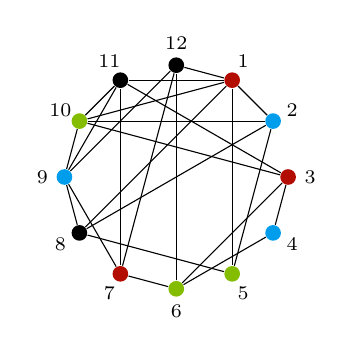
\begin{tikzpicture}
        \begin{scope}[every node/.style = {font=\scriptsize}]
        \newcount \myc
        \foreach \n in {1, 3, 7}{
            \myc=\n \advance\myc by -1 \multiply\myc by -360 \divide\myc by 12 \advance\myc by 60.0
            \node[anchor=center] (L\n) at (\the\myc:1.7) {\n};
            \node[anchor=center, circle, fill=uofgpillarbox, inner sep=2pt] (N\n) at (\the\myc:1.42) {};
        }
        \foreach \n in {2, 4, 9}{
            \myc=\n \advance\myc by -1 \multiply\myc by -360 \divide\myc by 12 \advance\myc by 60.0
            \node[anchor=center] (L\n) at (\the\myc:1.7) {\n};
            \node[anchor=center, circle, fill=uofgcobalt, inner sep=2pt] (N\n) at (\the\myc:1.42) {};
        }
        \foreach \n in {5, 6, 10}{
            \myc=\n \advance\myc by -1 \multiply\myc by -360 \divide\myc by 12 \advance\myc by 60.0
            \node[anchor=center] (L\n) at (\the\myc:1.7) {\n};
            \node[anchor=center, circle, fill=uofglawn, inner sep=2pt] (N\n) at (\the\myc:1.42) {};
        }
        \foreach \n in {8, 11, 12}{
            \myc=\n \advance\myc by -1 \multiply\myc by -360 \divide\myc by 12 \advance\myc by 60.0
            \node[anchor=center] (L\n) at (\the\myc:1.7) {\n};
            \node[anchor=center, circle, fill=black, inner sep=2pt] (N\n) at (\the\myc:1.42) {};
        }
        \draw (N1) -- (N2);
        \draw (N1) -- (N5);
        \draw (N1) -- (N8);
        \draw (N1) -- (N10);
        \draw (N1) -- (N11);
        \draw (N1) -- (N12);
        \draw (N2) -- (N5);
        \draw (N2) -- (N8);
        \draw (N2) -- (N10);
        \draw (N3) -- (N4);
        \draw (N3) -- (N6);
        \draw (N3) -- (N10);
        \draw (N3) -- (N11);
        \draw (N4) -- (N6);
        \draw (N5) -- (N8);
        \draw (N6) -- (N7);
        \draw (N6) -- (N12);
        \draw (N7) -- (N9);
        \draw (N7) -- (N11);
        \draw (N7) -- (N12);
        \draw (N8) -- (N9);
        \draw (N9) -- (N10);
        \draw (N9) -- (N11);
        \draw (N9) -- (N12);
        \draw (N10) -- (N11);
    \end{scope}
    \end{tikzpicture}

    \begin{itemize}
        \item Given a $k$-colouring of a subgraph, that subgraph cannot have a clique of more than
            $k$ vertices.
            \begin{itemize}
                \item Each colour class describes an at-most-one constraint.
            \end{itemize}
        \item This does \emph{not} follow from reverse unit propagation.
    \end{itemize}
\end{frame}

\begin{frame}[fragile]{Bounds Using Cutting Planes}
\tiny\begin{Verbatim}[commandchars=\\\{\},codes={\catcode`$=3\catcode`^=7}]
pseudo-Boolean proof version 1.0
f 41 0
o x7 x9 x12
u 1 ~x12 1 ~x7 >= 1 ;
u 1 ~x12 >= 1 ;
\textcolor{uofgcobalt}{* at most one [ x1 x3 x9 ]}
p \textcolor{uofgrose}{nonadj1_3} 2 * \textcolor{uofgrose}{nonadj1_9} + \textcolor{uofgrose}{nonadj3_9} + 3 d \hfill\textcolor{uofglawn}{$\rightsquigarrow$ tmp1}
p \textcolor{uofgrose}{obj1} \textcolor{uofgrose}{tmp1} +
u 1 ~x11 1 ~x10 >= 1 ; \hfill\textcolor{uofglawn}{$\rightsquigarrow$ b3}
\textcolor{uofgcobalt}{* at-most-one [ x1 x3 x7 ]}
p \textcolor{uofgrose}{nonadj1_3} 2 * \textcolor{uofgrose}{nonadj1_7} + \textcolor{uofgrose}{nonadj3_7} + 3 d \hfill\textcolor{uofglawn}{$\rightsquigarrow$ tmp2}
p \textcolor{uofgrose}{obj1} \textcolor{uofgrose}{tmp2} +
u 1 ~x11 >= 1 ; \hfill\textcolor{uofglawn}{$\rightsquigarrow$ b4}
o x1 x2 x5 x8 \hfill\textcolor{uofglawn}{$\rightsquigarrow$ obj2}
u 1 ~x8 1 ~x5 >= 1 ; \hfill\textcolor{uofglawn}{$\rightsquigarrow$ b5}
p \textcolor{uofgrose}{obj2} \textcolor{uofgrose}{nonadj1_9} +
u 1 ~x8 >= 1 ; \hfill\textcolor{uofglawn}{$\rightsquigarrow$ b6}
\textcolor{uofgcobalt}{* at-most-one [ x1 x3 x7 ] [ x2 x4 x9 ] [ x5 x6 x10 ]}
p \textcolor{uofgrose}{nonadj1_3} 2 * \textcolor{uofgrose}{nonadj1_7} + \textcolor{uofgrose}{nonadj3_7} + 3 d \hfill\textcolor{uofglawn}{$\rightsquigarrow$ tmp3}
p \textcolor{uofgrose}{obj2} \textcolor{uofgrose}{tmp3} +
p \textcolor{uofgrose}{nonadj2_4} 2 * \textcolor{uofgrose}{nonadj2_9} + \textcolor{uofgrose}{nonadj4_9} + 3 d \hfill\textcolor{uofglawn}{$\rightsquigarrow$ tmp4}
p \textcolor{uofgrose}{obj2} \textcolor{uofgrose}{tmp3} + \textcolor{uofgrose}{tmp4} +
p \textcolor{uofgrose}{nonadj5_6} 2 * \textcolor{uofgrose}{nonadj5_10} + \textcolor{uofgrose}{nonadj6_10} + 3 d \hfill\textcolor{uofglawn}{$\rightsquigarrow$ tmp5}
p \textcolor{uofgrose}{obj2} \textcolor{uofgrose}{tmp3} + \textcolor{uofgrose}{tmp4} + \textcolor{uofgrose}{tmp5} +
u >= 1 ; \hfill\textcolor{uofglawn}{$\rightsquigarrow$ done}
c \textcolor{uofgrose}{done} 0
\end{Verbatim}
\end{frame}

\begin{frame}{Results}
    \begin{itemize}
        \item Implemented in the Glasgow Subgraph Solver.
            \begin{itemize}
                \item Bit-parallel, can perform a colouring and recursive call in under a microsecond.
            \end{itemize}
        \item 59 of the 80 DIMACS instances take under 1,000 seconds to solve without logging.
        \item Produced and verified proofs for 57 of these 59 instances (the other two reached
            1TByte disk space).
        \item Mean slowdown from proof logging is 80.1 (due to disk I/O).
        \item Mean verification slowdown a further 10.1.
        \item Approximate implementation effort: one Masters student.
    \end{itemize}
\end{frame}

\begin{frame}{Maximum Clique in General}
    \begin{itemize}
        \item There are a lot of maximum clique algorithms:
            \begin{itemize}
                \item Different search orders.
                \item Different bound functions.
                \item Different data structures.
                \item Priming using local search.
            \end{itemize}
        \item Once you've implemented proof logging for one, the rest require very little effort.
    \end{itemize}
\end{frame}

\begin{frame}{Maximal Clique Enumeration}
    \begin{itemize}
        \item There are contradictory results for several graphs in the literature\ldots
        \item For proof logging:
            \begin{itemize}
                \item Maximality property is easily expressed in PB (``either take $v$, or at least
                    one of $v$'s neighbours'').
                \item Proof log every backtrack and every solution.
                \item No need to proof log the ``not set''.
            \end{itemize}
        \item This works for \emph{all} maximal clique algorithms.
        \item Implementation effort: roughly one day for someone who had never implemented
            any kind of proof logging before.
        \item Works for standard benchmark graphs of up to 10,000 vertices.
    \end{itemize}
\end{frame}

\begin{frame}[fragile]{Maximum Weight Clique}
    \begin{minipage}[c]{0.32\textwidth}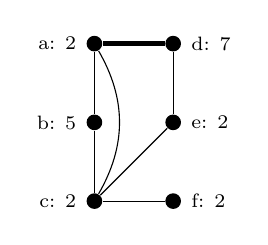
\begin{tikzpicture}[every node/.style = {font=\scriptsize}]
        \node[anchor=center, circle, fill=black, inner sep=2pt] (Na) at (0, 0) {};
        \node[anchor=center, left = 0cm of Na] {a: 2};

        \node[anchor=center, circle, fill=black, inner sep=2pt] (Nb) at (0, -1) {};
        \node[anchor=center, left = 0cm of Nb] {b: 5};

        \node[anchor=center, circle, fill=black, inner sep=2pt] (Nc) at (0, -2) {};
        \node[anchor=center, left = 0cm of Nc] {c: 2};

        \node[anchor=center, circle, fill=black, inner sep=2pt] (Nd) at (1, 0) {};
        \node[anchor=center, right = 0cm of Nd] {d: 7};

        \node[anchor=center, circle, fill=black, inner sep=2pt] (Ne) at (1, -1) {};
        \node[anchor=center, right = 0cm of Ne] {e: 2};

        \node[anchor=center, circle, fill=black, inner sep=2pt] (Nf) at (1, -2) {};
        \node[anchor=center, right = 0cm of Nf] {f: 2};

        \draw [ultra thick] (Na) -- (Nd);
        \draw (Na) -- (Nb);
        \draw (Na) to [out=300, in=60] (Nc);
        \draw (Nb) -- (Nc);
        \draw (Nc) -- (Ne);
        \draw (Nc) -- (Nf);
        \draw (Nd) -- (Ne);
    \end{tikzpicture}\end{minipage}\hfill\begin{minipage}[c]{0.55\textwidth}
\tiny\begin{Verbatim}[commandchars=\\\{\},codes={\catcode`$=3\catcode`^=7}]
pseudo-Boolean proof version 1.0
f 8 0
o xa xd \hfill\textcolor{uofglawn}{$\rightsquigarrow$ obj}
p \textcolor{uofgrose}{nonadja_e} 2 * \textcolor{uofgrose}{nonadja_f} + \textcolor{uofgrose}{nonadje_f} + 3 d 2 * \hfill\textcolor{uofglawn}{$\rightsquigarrow$ cc1}
p \textcolor{uofgrose}{nonadjb_d} 5 * \hfill\textcolor{uofglawn}{$\rightsquigarrow$ cc2}
p \textcolor{uofgrose}{nonadjc_d} 2 * \hfill\textcolor{uofglawn}{$\rightsquigarrow$ cc3}
p \textcolor{uofgrose}{obj} \textcolor{uofgrose}{cc1} + \textcolor{uofgrose}{cc2} + \textcolor{uofgrose}{cc3} + \hfill\textcolor{uofglawn}{$\rightsquigarrow$ done}
c \textcolor{uofgrose}{done} 0
\end{Verbatim}
\end{minipage}
\bigskip

    \begin{itemize}
        \item Colour classes have weights.
            \begin{itemize}
                \item Just multiply a colour class by its weight.
            \end{itemize}
        \item Vertices can split their weights between colour classes.
            \begin{itemize}
                \item That's fine, no changes needed.
            \end{itemize}
        \item Implementation effort: an afternoon, having seen roughly how it's done for unweighted
            cliques.
    \end{itemize}
\end{frame}

\section{Common Subgraph}

\begin{frame}{Maximum Common Subgraph}
    \centering
    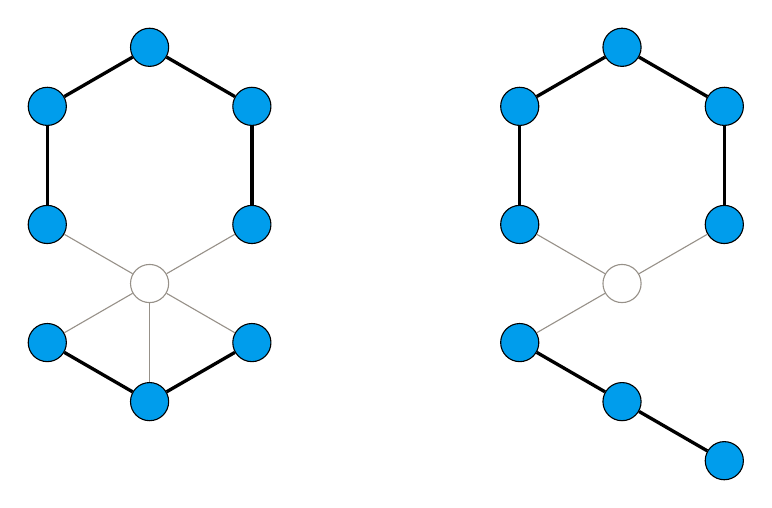
\begin{tikzpicture}
        \begin{scope}
            \node[draw, circle, fill=uofgcobalt, inner sep=2pt, font=\normalsize] (M1) at (90:1.5) {\phantom{0}};
            \node[draw, circle, fill=uofgcobalt, inner sep=2pt, font=\normalsize] (M2) at (150:1.5) {\phantom{0}};
            \node[draw, circle, fill=uofgcobalt, inner sep=2pt, font=\normalsize] (M3) at (30:1.5) {\phantom{0}};
            \node[draw, circle, fill=uofgcobalt, inner sep=2pt, font=\normalsize] (M4) at (210:1.5) {\phantom{0}};
            \node[draw, circle, fill=uofgcobalt, inner sep=2pt, font=\normalsize] (M5) at (330:1.5) {\phantom{0}};
            \node[draw, circle, draw=uofgsandstone!60, fill=white, inner sep=2pt, font=\normalsize] (M6) at (270:1.5) {\phantom{0}};
            \node[draw, circle, fill=uofgcobalt, inner sep=2pt, font=\normalsize] (M7) at ($(210:1.5) + (M6)$) {\phantom{0}};
            \node[draw, circle, fill=uofgcobalt, inner sep=2pt, font=\normalsize] (M8) at ($(330:1.5) + (M6)$) {\phantom{0}};
            \node[draw, circle, fill=uofgcobalt, inner sep=2pt, font=\normalsize] (M9) at ($(270:1.5) + (M6)$) {\phantom{0}};

            \draw [very thick] (M1) -- (M2);
            \draw [very thick] (M2) -- (M4);
            \draw [very thick] (M3) -- (M5);
            \draw [color=uofgsandstone!60] (M4) -- (M6);
            \draw [color=uofgsandstone!60] (M5) -- (M6);
            \draw [very thick] (M3) -- (M1);
            \draw [color=uofgsandstone!60] (M6) -- (M7);
            \draw [color=uofgsandstone!60] (M6) -- (M8);
            \draw [color=uofgsandstone!60] (M6) -- (M9);
            \draw [very thick] (M7) -- (M9);
            \draw [very thick] (M8) -- (M9);
        \end{scope}

        \begin{scope}[xshift=6cm]
            \node[draw, circle, fill=uofgcobalt, inner sep=2pt, font=\normalsize] (M1) at (90:1.5) {\phantom{0}};
            \node[draw, circle, fill=uofgcobalt, inner sep=2pt, font=\normalsize] (M2) at (150:1.5) {\phantom{0}};
            \node[draw, circle, fill=uofgcobalt, inner sep=2pt, font=\normalsize] (M3) at (30:1.5) {\phantom{0}};
            \node[draw, circle, fill=uofgcobalt, inner sep=2pt, font=\normalsize] (M4) at (210:1.5) {\phantom{0}};
            \node[draw, circle, fill=uofgcobalt, inner sep=2pt, font=\normalsize] (M5) at (330:1.5) {\phantom{0}};
            \node[draw, circle, draw=uofgsandstone!60, fill=white, inner sep=2pt, font=\normalsize] (M6) at (270:1.5) {\phantom{0}};
            \node[draw, circle, fill=uofgcobalt, inner sep=2pt, font=\normalsize] (M7) at ($(210:1.5) + (M6)$) {\phantom{0}};
            \node[draw, circle, fill=uofgcobalt, inner sep=2pt, font=\normalsize] (M8) at ($(270:1.5) + (M6)$) {\phantom{0}};
            \node[draw, circle, fill=uofgcobalt, inner sep=2pt, font=\normalsize] (M9) at ($(330:1.5) + (M8)$) {\phantom{0}};

            \draw [very thick] (M1) -- (M2);
            \draw [very thick] (M2) -- (M4);
            \draw [very thick] (M3) -- (M5);
            \draw [color=uofgsandstone!60] (M4) -- (M6);
            \draw [color=uofgsandstone!60] (M5) -- (M6);
            \draw [very thick] (M3) -- (M1);
            \draw [color=uofgsandstone!60] (M6) -- (M7);
            \draw [very thick] (M7) -- (M8);
            \draw [very thick] (M8) -- (M9);
        \end{scope}
    \end{tikzpicture}
\end{frame}

\begin{frame}{Maximum Common Connected Subgraph}
    \centering
    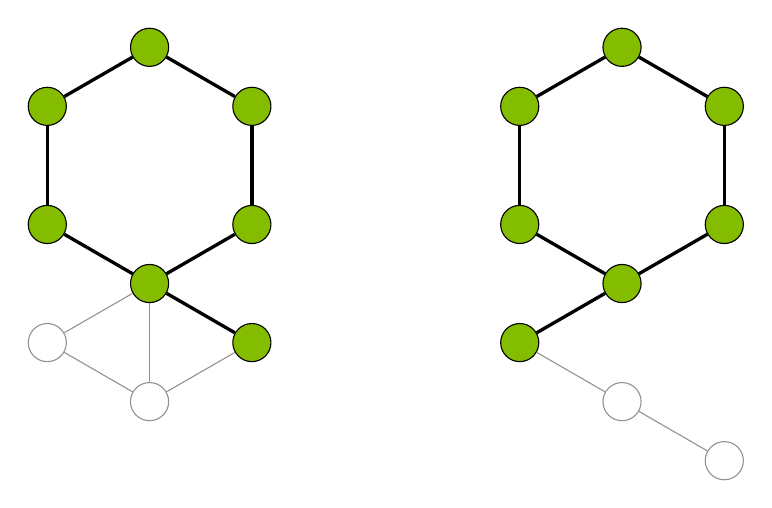
\begin{tikzpicture}
        \begin{scope}
            \node[draw, circle, fill=uofglawn, inner sep=2pt, font=\normalsize] (M1) at (90:1.5) {\phantom{0}};
            \node[draw, circle, fill=uofglawn, inner sep=2pt, font=\normalsize] (M2) at (150:1.5) {\phantom{0}};
            \node[draw, circle, fill=uofglawn, inner sep=2pt, font=\normalsize] (M3) at (30:1.5) {\phantom{0}};
            \node[draw, circle, fill=uofglawn, inner sep=2pt, font=\normalsize] (M4) at (210:1.5) {\phantom{0}};
            \node[draw, circle, fill=uofglawn, inner sep=2pt, font=\normalsize] (M5) at (330:1.5) {\phantom{0}};
            \node[draw, circle, fill=uofglawn, inner sep=2pt, font=\normalsize] (M6) at (270:1.5) {\phantom{0}};
            \node[draw, circle, draw=uofgsandstone!60, fill=white, inner sep=2pt, font=\normalsize] (M7) at ($(210:1.5) + (M6)$) {\phantom{0}};
            \node[draw, circle, fill=uofglawn, inner sep=2pt, font=\normalsize] (M8) at ($(330:1.5) + (M6)$) {\phantom{0}};
            \node[draw, circle, draw=uofgsandstone!60, fill=white, inner sep=2pt, font=\normalsize] (M9) at ($(270:1.5) + (M6)$) {\phantom{0}};

            \draw [very thick] (M1) -- (M2);
            \draw [very thick] (M2) -- (M4);
            \draw [very thick] (M3) -- (M5);
            \draw [very thick] (M4) -- (M6);
            \draw [very thick] (M5) -- (M6);
            \draw [very thick] (M3) -- (M1);
            \draw [color=uofgsandstone!60] (M6) -- (M7);
            \draw [very thick] (M6) -- (M8);
            \draw [color=uofgsandstone!60] (M6) -- (M9);
            \draw [color=uofgsandstone!60] (M7) -- (M9);
            \draw [color=uofgsandstone!60] (M8) -- (M9);
        \end{scope}

        \begin{scope}[xshift=6cm]
            \node[draw, circle, fill=uofglawn, inner sep=2pt, font=\normalsize] (M1) at (90:1.5) {\phantom{0}};
            \node[draw, circle, fill=uofglawn, inner sep=2pt, font=\normalsize] (M2) at (150:1.5) {\phantom{0}};
            \node[draw, circle, fill=uofglawn, inner sep=2pt, font=\normalsize] (M3) at (30:1.5) {\phantom{0}};
            \node[draw, circle, fill=uofglawn, inner sep=2pt, font=\normalsize] (M4) at (210:1.5) {\phantom{0}};
            \node[draw, circle, fill=uofglawn, inner sep=2pt, font=\normalsize] (M5) at (330:1.5) {\phantom{0}};
            \node[draw, circle, fill=uofglawn, inner sep=2pt, font=\normalsize] (M6) at (270:1.5) {\phantom{0}};
            \node[draw, circle, fill=uofglawn, inner sep=2pt, font=\normalsize] (M7) at ($(210:1.5) + (M6)$) {\phantom{0}};
            \node[draw, circle, draw=uofgsandstone!60, fill=white, inner sep=2pt, font=\normalsize] (M8) at ($(270:1.5) + (M6)$) {\phantom{0}};
            \node[draw, circle, draw=uofgsandstone!60, fill=white, inner sep=2pt, font=\normalsize] (M9) at ($(330:1.5) + (M8)$) {\phantom{0}};

            \draw [very thick] (M1) -- (M2);
            \draw [very thick] (M2) -- (M4);
            \draw [very thick] (M3) -- (M5);
            \draw [very thick] (M4) -- (M6);
            \draw [very thick] (M5) -- (M6);
            \draw [very thick] (M3) -- (M1);
            \draw [very thick] (M6) -- (M7);
            \draw [draw=uofgsandstone!60] (M7) -- (M8);
            \draw [draw=uofgsandstone!60] (M8) -- (M9);
        \end{scope}
    \end{tikzpicture}
\end{frame}


\begin{frame}{The McSplit Solver}
    \begin{itemize}
        \item A CP forward checker, but with different underlying data structures.
        \item All-different-except-$\bot$ as a bound function.
        \item Connected is handled by a combination of branching rules and propagation.
            \begin{itemize}
                \item Slightly awkward to encode in PB: requires dependent auxiliary variables.
                \item Reverse unit propagation handles it without help.
            \end{itemize}
    \end{itemize}
\end{frame}

\begin{frame}{Reduction to Clique}
    \centering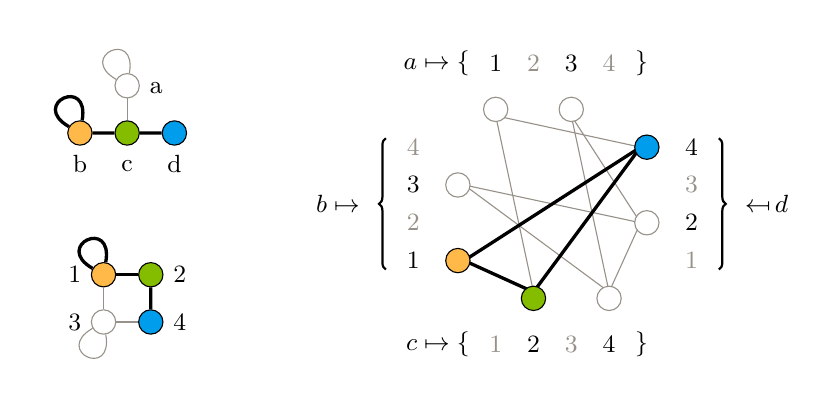
\begin{tikzpicture}[scale=0.30, font=\small]%{{{
        \begin{scope}
            \node[draw, circle, fill=white, draw=uofgsandstone!60, inner sep=0.5pt, font=\small] (Ma) at (2, 8) {\phantom{0}};
            \node[draw, circle, fill=uofgpumpkin, inner sep=0.5pt, font=\small] (Mb) at (0, 6) {\phantom{0}};
            \node[draw, circle, fill=uofglawn, inner sep=0.5pt, font=\small] (Mc) at (2, 6) {\phantom{0}};
            \node[draw, circle, fill=uofgcobalt, inner sep=0.5pt, font=\small] (Md) at (4, 6) {\phantom{0}};

            \node [right = 0 of Ma, font=\small] { \vphantom{0}a };
            \node [below = 0 of Mb, font=\small] { \vphantom{0}b };
            \node [below = 0 of Mc, font=\small] { \vphantom{0}c };
            \node [below = 0 of Md, font=\small] { \vphantom{0}d };

            \draw [very thick] (Mb) -- (Mc);
            \draw [very thick] (Mc) -- (Md);
            \draw [color=uofgsandstone!60] (Ma) -- (Mc);
            \draw [color=uofgsandstone!60] (Ma) to [out=150, in=80, looseness=8] (Ma);
            \draw [very thick] (Mb) to [out=150, in=80, looseness=8] (Mb);
        \end{scope}

        \begin{scope}[yshift=-2cm]
            \node[draw, circle, fill=uofgpumpkin, inner sep=0.5pt, font=\small] (M1) at (1, 2) {\phantom{0}};
            \node[draw, circle, fill=uofglawn, inner sep=0.5pt, font=\small] (M2) at (3, 2) {\phantom{0}};
            \node[draw, circle, fill=white, draw=uofgsandstone!60, inner sep=0.5pt, font=\small] (M3) at (1, 0) {\phantom{0}};
            \node[draw, circle, fill=uofgcobalt, inner sep=0.5pt, font=\small] (M4) at (3, 0) {\phantom{0}};

            \node [left = 0 of M1, font=\small] { \vphantom{0}1 };
            \node [right = 0 of M2, font=\small] { \vphantom{0}2 };
            \node [left = 0 of M3, font=\small] { \vphantom{0}3 };
            \node [right = 0 of M4, font=\small] { \vphantom{0}4 };

            \draw [very thick] (M1) -- (M2);
            \draw [very thick] (M2) -- (M4);
            \draw [color=uofgsandstone!60] (M3) -- (M4);
            \draw [color=uofgsandstone!60] (M1) -- (M3);

            \draw [color=uofgsandstone!60] (M3) to [out=280, in=210, looseness=8] (M3);
            \draw [very thick] (M1) to [out=150, in=80, looseness=8] (M1);
        \end{scope}

        \begin{scope}[xshift=15cm, yshift=-2cm]
            \node[draw, circle, fill=white, draw=uofgsandstone!60, inner sep=0.5pt, font=\small] (Ma1) at (2.6, 9) {\phantom{0}};
            \node[draw, circle, fill=white, draw=white, inner sep=0.5pt, font=\small] (Ma2) at (4.2, 9) {\phantom{0}};
            \node[draw, circle, fill=white, draw=uofgsandstone!60, inner sep=0.5pt, font=\small] (Ma3) at (5.8, 9) {\phantom{0}};
            \node[draw, circle, fill=white, draw=white, inner sep=0.5pt, font=\small] (Ma4) at (7.4, 9) {\phantom{0}};
            \node (La1) [above = 0.2cm of Ma1, font=\small] { \vphantom{0}1 };
            \node (La2) [above = 0.2cm of Ma2, font=\small, color=uofgsandstone!60] { \vphantom{0}2 };
            \node (La3) [above = 0.2cm of Ma3, font=\small] { \vphantom{0}3 };
            \node (La4) [above = 0.2cm of Ma4, font=\small, color=uofgsandstone!60] { \vphantom{0}4 };

            \node [left=0 of La1] { $a \mapsto \{$ };
            \node [right=0 of La4] { $\}$ };

            \node[draw, circle, fill=uofgpumpkin, inner sep=0.5pt, font=\small] (Mb1) at (1, 2.6) {\phantom{0}};
            \node[draw, circle, fill=white, draw=white, inner sep=0.5pt, font=\small] (Mb2) at (1, 4.2) {\phantom{0}};
            \node[draw, circle, fill=white, draw=uofgsandstone!60, inner sep=0.5pt, font=\small] (Mb3) at (1, 5.8) {\phantom{0}};
            \node[draw, circle, fill=white, draw=white, inner sep=0.5pt, font=\small] (Mb4) at (1, 7.4) {\phantom{0}};
            \node [left = 0.2cm of Mb1, font=\small] { \vphantom{0}1 };
            \node [left = 0.2cm of Mb2, font=\small, color=uofgsandstone!60] { \vphantom{0}2 };
            \node [left = 0.2cm of Mb3, font=\small] { \vphantom{0}3 };
            \node [left = 0.2cm of Mb4, font=\small, color=uofgsandstone!60] { \vphantom{0}4 };

            \draw [decorate, decoration={brace, raise=0.8cm}, thick] (Mb1.south west) -- (Mb4.north west) node [midway, left=1cm] { $b \mapsto$ };

            \node[draw, circle, fill=white, draw=white, inner sep=0.5pt, font=\small] (Mc1) at (2.6, 1) {\phantom{0}};
            \node[draw, circle, fill=uofglawn, inner sep=0.5pt, font=\small] (Mc2) at (4.2, 1) {\phantom{0}};
            \node[draw, circle, fill=white, draw=white, inner sep=0.5pt, font=\small] (Mc3) at (5.8, 1) {\phantom{0}};
            \node[draw, circle, fill=white, draw=uofgsandstone!60, inner sep=0.5pt, font=\small] (Mc4) at (7.4, 1) {\phantom{0}};
            \node (Lc1) [below = 0.2cm of Mc1, font=\small, color=uofgsandstone!60] { \vphantom{0}1 };
            \node (Lc2) [below = 0.2cm of Mc2, font=\small] { \vphantom{0}2 };
            \node (Lc3) [below = 0.2cm of Mc3, font=\small, color=uofgsandstone!60] { \vphantom{0}3 };
            \node (Lc4) [below = 0.2cm of Mc4, font=\small] { \vphantom{0}4 };

            \node [left=0 of Lc1] { $c \mapsto \{$ };
            \node [right=0 of Lc4] { $\}$ };

            \node[draw, circle, fill=white, draw=white, inner sep=0.5pt, font=\small] (Md1) at (9, 2.6) {\phantom{0}};
            \node[draw, circle, fill=white, draw=uofgsandstone!60, inner sep=0.5pt, font=\small] (Md2) at (9, 4.2) {\phantom{0}};
            \node[draw, circle, fill=white, draw=white, inner sep=0.5pt, font=\small] (Md3) at (9, 5.8) {\phantom{0}};
            \node[draw, circle, fill=uofgcobalt, inner sep=0.5pt, font=\small] (Md4) at (9, 7.4) {\phantom{0}};
            \node [right = 0.2cm of Md1, font=\small, color=uofgsandstone!60] { \vphantom{0}1 };
            \node [right = 0.2cm of Md2, font=\small] { \vphantom{0}2 };
            \node [right = 0.2cm of Md3, font=\small, color=uofgsandstone!60] { \vphantom{0}3 };
            \node [right = 0.2cm of Md4, font=\small] { \vphantom{0}4 };

            \draw [decorate, decoration={brace, raise=0.8cm}, thick] (Md4.north east) -- (Md1.south east) node [midway, right=1cm] { $\reflectbox{\ensuremath{\mapsto}}\, d$ };

            \begin{scope}[on background layer]
                \draw [draw=uofgsandstone!60] ($(Ma1.south)!0.5!(Ma1)$) -- ($(Md4.west)!0.5!(Md4)$);
                \draw [draw=uofgsandstone!60] ($(Ma1.south)!0.5!(Ma1)$) -- ($(Mc2.north)!0.5!(Mc2)$);
                \draw [draw=uofgsandstone!60] ($(Ma3.south)!0.5!(Ma3)$) -- ($(Mc4.north)!0.5!(Mc4)$);
                \draw [draw=uofgsandstone!60] ($(Mb3.east)!0.5!(Mb3)$) -- ($(Mc4.north)!0.5!(Mc4)$);
                \draw [draw=uofgsandstone!60] ($(Md2.west)!0.5!(Md2)$) -- ($(Mc4.north)!0.5!(Mc4)$);
                \draw [draw=uofgsandstone!60] ($(Md2.west)!0.5!(Md2)$) -- ($(Ma3.south)!0.5!(Ma3)$);
                \draw [draw=uofgsandstone!60] ($(Md2.west)!0.5!(Md2)$) -- ($(Mb3.east)!0.5!(Mb3)$);
                \draw [very thick] ($(Mb1.east)!0.5!(Mb1)$) -- ($(Mc2.north)!0.5!(Mc2)$);
                \draw [very thick] ($(Mb1.east)!0.5!(Mb1)$) -- ($(Md4.west)!0.5!(Md4)$);
                \draw [very thick] ($(Mc2.north)!0.5!(Mc2)$) -- ($(Md4.west)!0.5!(Md4)$);
        \end{scope}
        \end{scope}

    \end{tikzpicture}

    \begin{itemize}
        \item We can encode this reduction using cutting planes rules. No need for a different OPB
            file.
        \item The clique solver does not need to be modified.
        \item This even works for connectivity.
    \end{itemize}
\end{frame}

\begin{frame}{Results}
    \begin{itemize}
        \item McSplit: implemented in a day by someone with no prior proof logging experience.
            \begin{itemize}
                \item 16,300 instances, proof logging slowdowns of 67.0 and 298.9.
                \item McSplit can make five million recursive calls per second.
                \item Verification slowdown of 13.4 and 21.6.
            \end{itemize}
        \item Clique: implemented alongside the algorithm in under a day.
            \begin{itemize}
                \item 11,400 instances verified, proof logging slowdown of 28.6 and 39.7.
                \item Verification slowdown of 11.3 and 73.1.
                \item Caught a bug in the implementation that testing had missed.
            \end{itemize}
    \end{itemize}
\end{frame}

\section{Subgraph Isomorphism}

\begin{frame}{Subgraph Isomorphism}
    \only<1-2>{
    \centering
    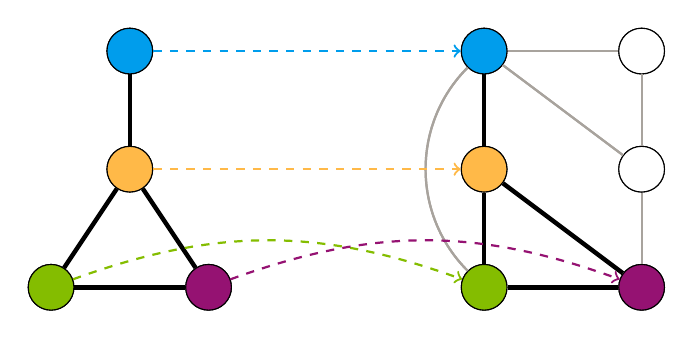
\begin{tikzpicture}
        \node <1> [draw, circle, fill=white, inner sep=4pt, font=\bfseries] (Na) at (1,  0) {\vphantom{1}};
        \node <1> [draw, circle, fill=white, inner sep=4pt, font=\bfseries] (Nb) at (1, -1.5) {\vphantom{1}};
        \node <1> [draw, circle, fill=white, inner sep=4pt, font=\bfseries] (Nc) at (0, -3) {\vphantom{1}};
        \node <1> [draw, circle, fill=white, inner sep=4pt, font=\bfseries] (Nd) at (2, -3) {\vphantom{1}};

        \node <2> [draw, circle, fill=uofgcobalt, inner sep=4pt, font=\bfseries] (Na) at (1,  0) {\vphantom{1}};
        \node <2> [draw, circle, fill=uofgpumpkin, inner sep=4pt, font=\bfseries] (Nb) at (1, -1.5) {\vphantom{1}};
        \node <2> [draw, circle, fill=uofglawn, inner sep=4pt, font=\bfseries] (Nc) at (0, -3) {\vphantom{1}};
        \node <2> [draw, circle, fill=uofgthistle, inner sep=4pt, font=\bfseries] (Nd) at (2, -3) {\vphantom{1}};

        \draw [ultra thick] (Na) -- (Nb);
        \draw [ultra thick] (Nb) -- (Nc);
        \draw [ultra thick] (Nc) -- (Nd);
        \draw [ultra thick] (Nb) -- (Nd);

        \node <1> [draw, circle, fill=white, inner sep=4pt, font=\bfseries] (N1) at (5.5,  0) {\vphantom{1}};
        \node <1> [draw, circle, fill=white, inner sep=4pt, font=\bfseries] (N2) at (7.5,  0) {\vphantom{1}};
        \node <1> [draw, circle, fill=white, inner sep=4pt, font=\bfseries] (N3) at (5.5, -1.5) {\vphantom{1}};
        \node <1> [draw, circle, fill=white, inner sep=4pt, font=\bfseries] (N4) at (7.5, -1.5) {\vphantom{1}};
        \node <1> [draw, circle, fill=white, inner sep=4pt, font=\bfseries] (N5) at (5.5, -3) {\vphantom{1}};
        \node <1> [draw, circle, fill=white, inner sep=4pt, font=\bfseries] (N6) at (7.5, -3) {\vphantom{1}};

        \node <2> [draw, circle, fill=uofgcobalt, inner sep=4pt, font=\bfseries] (N1) at (5.5,  0) {\vphantom{1}};
        \node <2> [draw, circle, fill=white, inner sep=4pt, font=\bfseries] (N2) at (7.5,  0) {\vphantom{1}};
        \node <2> [draw, circle, fill=uofgpumpkin, inner sep=4pt, font=\bfseries] (N3) at (5.5, -1.5) {\vphantom{1}};
        \node <2> [draw, circle, fill=white, inner sep=4pt, font=\bfseries] (N4) at (7.5, -1.5) {\vphantom{1}};
        \node <2> [draw, circle, fill=uofglawn, inner sep=4pt, font=\bfseries] (N5) at (5.5, -3) {\vphantom{1}};
        \node <2> [draw, circle, fill=uofgthistle, inner sep=4pt, font=\bfseries] (N6) at (7.5, -3) {\vphantom{1}};

        \draw <1> [thick, color=uofgsandstone!50] (N1) -- (N2);
        \draw <1> [thick, color=uofgsandstone!50] (N1) -- (N3);
        \draw <1> [thick, color=uofgsandstone!50] (N1) -- (N4);
        \draw <1> [thick, color=uofgsandstone!50] (N2) -- (N4);
        \draw <1> [thick, color=uofgsandstone!50] (N3) -- (N5);
        \draw <1> [thick, color=uofgsandstone!50] (N3) -- (N6);
        \draw <1> [thick, color=uofgsandstone!50] (N4) -- (N6);
        \draw <1> [thick, color=uofgsandstone!50] (N5) -- (N6);
        \draw <1> [thick, color=uofgsandstone!50] (N1) to [in=135, out=225] (N5);

        \draw <2> [thick, color=uofgsandstone!50] (N1) -- (N2);
        \draw <2> [ultra thick] (N1) -- (N3);
        \draw <2> [thick, color=uofgsandstone!50] (N1) -- (N4);
        \draw <2> [thick, color=uofgsandstone!50] (N2) -- (N4);
        \draw <2> [ultra thick] (N3) -- (N5);
        \draw <2> [ultra thick] (N3) -- (N6);
        \draw <2> [thick, color=uofgsandstone!50] (N4) -- (N6);
        \draw <2> [ultra thick] (N5) -- (N6);
        \draw <2> [thick, color=uofgsandstone!50] (N1) to [in=135, out=225] (N5);

        \draw <2> [thick, dashed, color=uofgcobalt, arrows=->] (Na) to (N1);
        \draw <2> [thick, dashed, color=uofgpumpkin, arrows=->] (Nb) to (N3);
        \draw <2> [thick, dashed, color=uofglawn, arrows=->] (Nc) to [out=20, in=160] (N5);
        \draw <2> [thick, dashed, color=uofgthistle, arrows=->] (Nd) to [out=20, in=160] (N6);
    \end{tikzpicture}}
\end{frame}

\begin{frame}[t]{Subgraph Isomorphism in Pseudo-Boolean Form}
    \begin{itemize}
        \item Each pattern vertex must be mapped to exactly one target vertex: \begin{align*}
    \sum_{t \in \vertexset(T)} x_{p{,}t}  & = 1 && p \in \vertexset(P)
\end{align*}
\item Injectivity, each target vertex may be used at most once:\begin{align*}
    \sum_{p \in \vertexset(P)} -x_{p{,}t} & \ge -1 && t \in \vertexset(T)
\end{align*}
\item Adjacency constraints, if a vertex $p$ is mapped to a vertex $t$, then every vertex in the
neighbourhood of $p$ must be mapped to a vertex in the neighbourhood of $t$:\begin{align*}
    \overline{x}_{p{,}t} + \sum_{u \in \neighbourhood(t)} x_{q{,}u} & \ge 1 && p \in \vertexset(P),~q \in \neighbourhood(p),~t \in \vertexset(T)
\end{align*}
    \end{itemize}
\end{frame}

\begin{frame}[fragile]{Degree Reasoning in Cutting Planes}
    \only<1>{
    \begin{itemize}
        \item A pattern vertex $p$ of degree $\degree(p)$ can never be mapped to a target vertex $t$ of degree
$\degree(p)-1$ or lower in any subgraph isomorphism.
\item Suppose $\neighbourhood(p) = \{ q, r, s \}$ and $\neighbourhood(t) = \{ u, v \}$.
\item We wish to derive $\overline{x}_{p{,t}} \ge 1$.
    \end{itemize}}\only<2>{
    \begin{itemize}
        \item We have the three adjacency constraints,
\begin{align*}
    \overline{x}_{p{,}t} + x_{q{,}u} + x_{q{,}v} & \ge 1 \\
    \overline{x}_{p{,}t} + x_{r{,}u} + x_{r{,}v} & \ge 1 \\
    \overline{x}_{p{,}t} + x_{s{,}u} + x_{s{,}v} & \ge 1
\end{align*}
\item Their sum is
\begin{align*}
    3 \overline{x}_{p{,}t} + x_{q{,}u} + x_{q{,}v}
    + x_{r{,}u} + x_{r{,}v}
    + x_{s{,}u} + x_{s{,}v} & \ge 3
\end{align*}\end{itemize}}\only<3>{
    \begin{itemize}
\item Continuing with the sum
\begin{align*}
    3 \overline{x}_{p{,}t} + x_{q{,}u} + x_{q{,}v}
    + x_{r{,}u} + x_{r{,}v}
    + x_{s{,}u} + x_{s{,}v} & \ge 3
\end{align*}
        \item Due to injectivity, at most one of $x_{q{,}u}$, $x_{r{,}u}$, and $x_{s{,}u}$
can be true, and similarly for $v$.
\item Add both these injectivity constraints, getting \[
    3 \overline{x}_{p{,}t}
    + \sum_{p \in \vertexset(P) \setminus \{q, r, s\}} -x_{p{,}u}
    + \sum_{p \in \vertexset(P) \setminus \{q, r, s\}} -x_{p{,}v}
    \ge 1\]
    \end{itemize}
}\only<4>{
    \begin{itemize}
\item Continuing with the sum of sums \[
    3 \overline{x}_{p{,}t}
    + \sum_{p \in \vertexset(P) \setminus \{q, r, s\}} -x_{p{,}u}
    + \sum_{p \in \vertexset(P) \setminus \{q, r, s\}} -x_{p{,}v}
    \ge 1\]
\item Add the literal axioms $x_i \ge 0$ to get \[
    3 \overline{x}_{p{,}t} \ge 1\]
\item Divide by 3 to get the desired \[
    \overline{x}_{p{,}t} \ge 1\]
    \end{itemize}
}\begin{onlyenv}<5>
\begin{Verbatim}
p 18 19 + 20 +      * sum adj constraints
  12 + 13 +         * sum inj constraints
  xp_u + xp_v +     * cancel stray xp_*
  xo_u + xo_v +     * cancel stray xo_*
  3 d 0             * divide, and we're done
e -1 1 ~xp_t >= 1 ; * check what we just did
\end{Verbatim}
\end{onlyenv}\begin{onlyenv}<6>
\begin{Verbatim}
p 18 19 + 20 +      * sum adj constraints
  12 + 13 + 0       * sum inj constraints
j -1 1 ~xp_t >= 1 ; * and simplify the above
\end{Verbatim}
\end{onlyenv}
\end{frame}

\begin{frame}{Other Forms of Reasoning}
    \begin{itemize}
        \item We can also do:
            \begin{itemize}
                \item All-different.
                \item Distance filtering.
                \item Neighbourhood degree sequences.
                \item Path filtering.
                \item Supplemental graphs.
            \end{itemize}
        \item Proof steps are ``efficient'' using cutting planes.
    \end{itemize}
\end{frame}

\begin{frame}{It Works!}
    \begin{itemize}
        \item Able to produce and verify Glasgow Subgraph Solver proofs for medium-sized instances
            for the first time.
        \item Can't guarantee the solver is free of bugs, but if it ever outputs an incorrect
            answer, we will detect it.
        \item No changes to the reasoning carried out by the solver.
    \end{itemize}
\end{frame}

\begin{frame}{Problem Instances}
    \begin{itemize}
        \item The Pseudo-Boolean models can be large: had to restrict to instances with no more than
            260 vertices in the target graph.
        \item Took enumeration instances which could be solved without proof logging in under ten seconds.
        \item 1,227 instances from Solnon's benchmark collection:
            \begin{itemize}
                \item 789 unsatisfiable, up to 50,635,140 solutions in the rest.
                \item 498 instances solved without guessing.
                \item Hardest solved satisfiable and unsatisfiable instances required 53,605,482 and
                    2,074,386 recursive calls.
            \end{itemize}
    \end{itemize}
\end{frame}

\begin{frame}{Hard Disks Make This Quite Slow}
    \begin{center}
        \only<1>{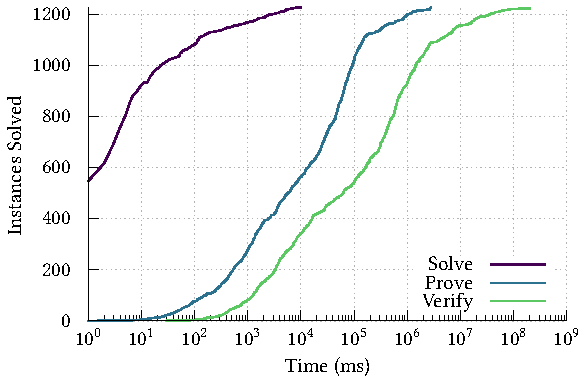
\includegraphics{gen-graph-cumulative.pdf}}%
        \only<2>{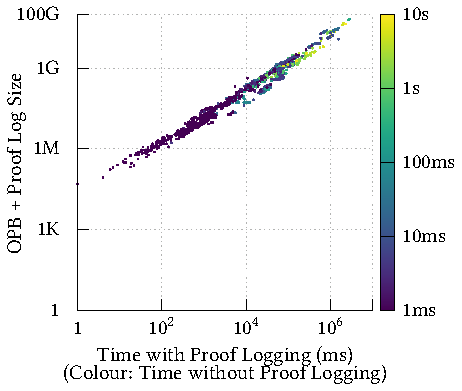
\includegraphics{gen-graph-write-speed.pdf}}%
    \end{center}
\end{frame}

\section{Constraint Programming}

\begin{frame}{Constraint Programming}
    \begin{itemize}
        \item Integer domains.
        \item Rich constraints with different propagation algorithms.
        \item Need to reformulate constraints and models.
    \end{itemize}
\end{frame}

\begin{frame}{Extension Variables}
    \begin{itemize}
        \item Given a pseudo-Boolean constraint $C$ and a fresh variable $y$, introduce \[ y
            \leftrightarrow C \]
        \item Straightforward use of redundance-based strengthening.
    \end{itemize}
\end{frame}

\begin{frame}{Expressing CP Variables in Pseudo-Boolean Form}
    \begin{itemize}
        \item Given $X \in \{ 1, 2, 3 \}$, create $x_{{=}1}$, $x_{{=}2}$ and $x_{{=}3}$?
        \item Would also want $x_{{\ge}1}$ and $x_{{\ge}2}$ for convenience.
        \item Doesn't work for large domains whose bounds are trimmed during search.
    \end{itemize}
\end{frame}

\begin{frame}{Binary Encodings?}
    \begin{itemize}
        \item Given $A$ with domain $\{ -3 \ldots 9 \}$, how about
\begin{align*}
    -32 a_{{\operatorname{neg}}} + 1 a_{{\operatorname{b}}0} + 2 a_{{\operatorname{b}}1} + 4
    a_{{\operatorname{b}}2} + 8 a_{{\operatorname{b}}3} + 16 a_{{\operatorname{b}}4} &\ge -3
    \textnormal{~and}\\
    32 a_{{\operatorname{neg}}} + -1 a_{{\operatorname{b}}0} + -2 a_{{\operatorname{b}}1} +
    -4 a_{{\operatorname{b}}2} + -8 a_{{\operatorname{b}}3} + -16 a_{{\operatorname{b}}4} &\ge -9
    \textnormal{.}
\end{align*}
        \item Weakly propagating, but that doesn't matter.
        \item Really annoying for proofs.
    \end{itemize}
\end{frame}

\begin{frame}{Lazily Introducing Direct Variables}
    \begin{itemize}
        \item Go with the binary encoding.
        \item Whenever we propagate a value or bounds, introduce $x_{{\ge}i}$ and $x_{{=}i}$
            as extension variables.
        \item This works because for large domains, most values are never used.
    \end{itemize}
\end{frame}

\begin{frame}{Propagators}
    \begin{itemize}
        \item All different, linear inequalities: cutting planes.
        \item Table, absolute value, minimum / maximum: reverse unit propagation.
        \item Element, GAC linear equalities: reformulation then reverse unit propagation.
        \item Not equals: lazy reformulation.
    \end{itemize}
\end{frame}

\begin{frame}{Reformulation}
    \begin{itemize}
        \item Gratuitous use of extension variables.
        \item Sufficient for, e.g.\ tabulation of constraints.
        \item Also allows for more compact not-equals on large domains.
    \end{itemize}
\end{frame}

\begin{frame}{Symmetries}
    \begin{itemize}
        \item We could do proof logging for symmetry constraints, without including them in the OPB
            file.
    \end{itemize}
\end{frame}

\section{What's Next?}

%%%\begin{frame}{Redundance-Based Strengthening}
%%%\end{frame}
%%%
%%%\begin{frame}{Dominance and Symmetry}
%%%\end{frame}

\begin{frame}{Open Problems and Ongoing Work}
    \begin{itemize}
        \item Verification:
            \begin{itemize}
                \item A formally verified verifier.
                \item Verifying pseudo-Boolean encodings.
                \item Performance.
            \end{itemize}
        \item Proof-related:
            \begin{itemize}
                \item ``Lemmas'', or substitution proofs?
                \item Counting that isn't just enumeration.
                \item Approximate counting, uniform sampling, etc? Pareto fronts?
                \item Proof trimming or minimisation?
            \end{itemize}
        \item Things to proof log:
            \begin{itemize}
                \item Symmetric explanation learning.
                \item The 400 remaining global constraints I've not done yet.
                \item Every single dedicated solving algorithm ever.
            \end{itemize}
        \item Beyond proofs:
            \begin{itemize}
                \item Proof mining for experimental algorithmics?
            \end{itemize}
    \end{itemize}
\end{frame}

{
    \usebackgroundtemplate{
        \tikz[overlay, remember picture]
        \node[at=(current page.south), anchor=south, inner
        sep=0pt]{\includegraphics[keepaspectratio=true, width=\paperwidth]{background2.jpg}};
    }

    \begin{frame}[plain,noframenumbering]
        \begin{tikzpicture}[remember picture, overlay]
            \node at (current page.north west) {
                \begin{tikzpicture}[remember picture, overlay]
                    \fill [fill=uofguniversityblue, anchor=north west] (0, 0) rectangle (\paperwidth, -2.8cm);
                \end{tikzpicture}
            };

            \node (logo) [anchor=north east, shift={(-0.6cm,-0.2cm)}] at (current page.north east) {
                
\includegraphics[keepaspectratio=true,scale=0.5]{UoG_keyline.pdf}
            };

            \node (logo2) [anchor=north, below=0.2cm of logo.south] {
                
\includegraphics[keepaspectratio=true,scale=0.1]{RAEngWhite.pdf}
            };

            \coordinate (logos) at ($(logo.south)!0.5!(logo2.north)$);

            \node [anchor=west, xshift=0.2cm] at (current page.west |- logos) {
                \begin{minipage}{0.60\paperwidth}\raggedright
                    \textcolor{white}{\url{https://ciaranm.github.io/}} \\[0.3cm]
                    \textcolor{white}{\href{mailto:ciaran.mccreesh@glasgow.ac.uk}{\nolinkurl{ciaran.mccreesh@glasgow.ac.uk}}}
                \end{minipage}
            };
        \end{tikzpicture}
    \end{frame}
}

\end{document}

